\chapter{MATCH: A Decentralized Middleware for Fair Matchmaking In Peer-to-Peer Markets}
\label{chapter:match}

\emph{
	Order matchmaking is a core enabling element for electronic markets and online economy.
	A common approach to order matchmaking is the deployment of proprietary solutions, controlled by the market operators.
	This approach raises fairness concerns as market operators effectively have the capability to discriminate specific users when matching their orders.
	Blockchain technology has been proposed to enable transparent, open matchmaking solutions without a trusted operator.
	In practice, however, blockchain technology does not provide the required performance, in terms of transaction throughput, for fast order matching across many domains. }
	
\emph{
	In this chapter we present MATCH, a decentralized middleware for fair order matchmaking.
	By decoupling the dissemination of potential matches from the negotiation of trade agreements, MATCH empowers end-users to make their own educated decisions and to engage in direct negotiations with trade partners.
	This approach makes MATCH resilient against matchmakers that pursue selfish interests, a severe issue with centralized matchmaking.
	We implement MATCH and evaluate our middleware using real-world ride-hailing and asset trading workloads.
	It is demonstrated that MATCH maintains high matching quality, even in the presence of malicious matchmakers.
	Further, we show that the bandwidth, memory usage, and order fulfil latency of MATCH is orders of magnitude lower compared to matchmaking on an Ethereum blockchain. }

\newpage

\section{Introduction}
\label{sec:introduction}

The deployment of peer-to-peer markets by companies operating in the sharing economy has been hailed to boost the global economy~\cite{malhotra2014dark}.
Beyond the promises of increased economic welfare, the broader appeal of the sharing economy also lies with the development of new modes for the sharing of unused or underutilized assets, such as cars and houses. %, not unlike other collaborative mechanisms such as crowdfunding and open-source software development. %Reference. Benkler, Y., 2006. The Wealth of Networks: How Social Production Transforms Markets and Freedom, http://benkler.org/Benkler_Wealth_Of_Networks.pdf.
%While there is no single definition for the sharing economy, it can be considered as an umbrella term for novel technology-enabled peer-to-peer markets, enabling new types of interactions on a global scale.
%It has been suggested that the key defining characteristics of sharing economy are markets enabling direct peer-to-peer exchange or rent of under-utilized assets and resources.
%Given the inclusive character of the sharing economy label, the estimates of its size and impact vary. 
Estimations on the impact of the sharing economy suggest an increase in global revenue from \$14 billion in 2014 to \$335 billion by 2025, partially enabled by major platforms such as Uber (ride-hailing) and Airbnb (house-sharing)~\cite{pwcsharingeconomy}. %Reference. PricewaterhouseCoopers. (2015). Consumer Intelligence Series "The Sharing Economy", https://www.pwc.com/us/en/technology/publications/assets/pwc-consumer-intelligence-series-the-sharing-economy.pdf
%Major companies in the sharing economy are Uber (ride-hailing) and Airbnb (house-sharing).

The effect of these platforms on peer-to-peer markets, however, is not unequivocal.
It has been argued that market operators exploit their prominent position and charge high transaction fees for their role as intermediary~\cite{schor2016debating}. %Reference.  (Shapiro 2020) https://onlinelibrary.wiley.com/doi/abs/10.1111/ntwe.12160 
Market operators gain unprecedented power through the control of all the key enabling elements for electronic marketplaces, including settlement, arbitrage, and matchmaking~\cite{oecd2019,pepper2019,azevedo2016}.
%These developments stand in stark contrast with the promises of early peer-to-peer markets, that were envisioned as the enabler for open, fair, and competitive ecosystems~\cite{trastour2002}.
%Currently, however, such markets are mostly enabled by opaque, proprietary matchmaking mechanisms provided by the market operator %Reference. (Shapiro 2020)
The latter element is of particular interest as at the dawn of e-commerce matchmaking solutions were envisioned to create open, fair, and competitive markets on the Internet~\cite{trastour2002}.

Matchmaking in electronic markets can be considered as the process of mediating between supply and demand~\cite{veit2002multi}.
Currently, centralized matchmaking is the approach taken by most commercial market operators~\cite{azevedo2016,oecd2019}.
With centralized matchmaking, market operators deploy proprietary servers that are optimized to efficiently match new buy and sell orders with existing ones within a specific domain.
A key advantage of centralized matchmaking is that the market operator can match incoming orders with the (current) best compatible order since they maintain all market information.
%This approach also enables more simple software integration with other domain-specific services provided by the market operator.

Unfortunately, this also enables market operators to exploit the marketplace through the practices of unfair matchmaking to increase intermediary revenues~\cite{hannak2014}.
Manipulation in the matchmaking process was exposed through analysis of different e-commerce platforms and financial exchanges~\cite{oecd2019,mavroudis2019libra}.
%The scale of this problem is highlighted by the current antitrust investigation into Amazon’s suspected unfair treatment of customers by the European Commission ~\cite{ec2019}.
%It has been also argued that these developments not only introduce unfair competition in e-commerce but can also hurt the effectiveness of emerging peer-to-peer markets. %Reference. (Callo) https://digitalcommons.law.uw.edu/cgi/viewcontent.cgi?article=1046&context=faculty-articles
An emblematic example of this issue is the practices of Uber, implementing price discrimination and phantom matches to manipulate the behaviour of users~\cite{calo2017taking}. %Reference. (Shapiro) 
It has recently been demonstrated through experiments that the matchmaking algorithm of Uber undermines revenues of drivers to the advantages of the platform operator~\cite{bokanyi2019ride}.
As researchers point out, unfair matchmaking is a complex, multilayered issue that can not be mitigated only with algorithmic adjustments~\cite{bokanyi2019ride}.
We suggest that this problem requires a next step towards a different approach to matchmaking in peer-to-peer markets.

It is technologically feasible to have market participants carry out the matchmaking process themselves, without trusted operator.
In particular, blockchain technology provides the means to record and match market orders on a distributed ledger~\cite{subramanian2017decentralized}.
Smart contracts, self-executing programs stored on a blockchain, are capable of executing the matchmaking logic~\cite{luu2016making}.
Even though it seems like an appealing solution to fairness issues, the consensus algorithm managing the blockchain ledger is vulnerable to various attacks against fairness, specifically, \emph{transaction re-ordering} and \emph{front-running}~\cite{eskandari2019,kolluri2018,judmayer2019}.
These attacks effectively allow consensus participants to influence how specific orders are matched.
In addition to these threats, scalability issues inherent to all the blockchain protocols based on a global consensus carry significant limitations on the speed of matchmaking, as we will experimentally show in Section~\ref{sec:experiments_ethereum}~\cite{daian2019}.

%Currently, most of these advancements aim to provide decentralized alternatives to one of the key building blocks of e-commerce: settlement.%Reference. 
%However, decentralized settlement is not sufficient to ensure fair markets~\cite{pesch2019fictions}. %Reference. https://journals.sagepub.com/doi/full/10.1177/0306312719838339
%We suggest that an accompanying approach for decentralized matchmaking is the next logic step towards fair peer-to-peer markets.

The ineffectiveness of matchmaking on a blockchain is also identified by various decentralized exchanges that are operated by a blockchain, also called DEXes~\cite{eskandari2019,warren20170x,idex}.
%At the moment there are little to none solutions providing fair matchmaking in different markets.
In response, these DEXes opt for a federated approach where any participant can host a matchmaking server and can act as a matchmaker.
In practice, most orders in these DEXes are managed by servers that are under the control of the exchange operator and therefore still carry limitations on the achievable level of fairness desirable on such markets.

In summary, there is a dilemma of choice between two desirable properties of matchmaking mechanisms.
%These contradictions effectively create a dilemma of choice 
\emph{Efficiency} of matchmaking achievable through the concentration of orders by a trusted central party, versus provable \emph{fairness} of matchmaking achievable with the transparency of decentralized on-chain matchmaking.
We argue, however, that this dilemma does not present an insurmountable obstacle for the implementation of efficient and fair matchmaking solutions.

\textbf{Contributions.}
We present MATCH, a decentralized middleware for fair matchmaking in peer-to-peer markets.
Our solution is based on the principle of strictly decoupling the matching process from the negotiation of trade agreements.
Our first contribution is the MATCH protocol (Section~\ref{sec:protocol}) where any user can act as a matchmaker for others.
Matchmakers store open orders created by users, match incoming orders with existing ones, and inform order creators about potential matches.
Users then engage in trade negotiation with prospective counterparties.
This approach makes MATCH highly resistant against matchmakers which deviate from a standard matching algorithm. 
The second contribution is the generic MATCH middleware architecture (Section~\ref{sec:architecture}).
MATCH does not rely on the specifications of orders, and is therefore re-usable across different trading domains.
%Order creators disseminate a new order to multiple matchmakers while avoiding network- wide replication of orders.

%We evaluate MATCH using workloads for ride-hailing and asset trading, reconstructed from real world traces.
We devise the first decentralized and fair alternative to the Uber ride-hailing market (Section~\ref{sec:taxi_experiments}), to the best knowledge of the authors.
%We consider ride-hailing (Section~\ref{sec:taxi_experiments}) as a paradigmatic case to demonstrate how fair matchmaking can be achieved without market operator, even when the majority of drivers actively prioritize their own ride services during matchmaking.
Even when 75\% of all drivers prioritize their own ride services during matchmaking, negotiated matches in our market maintain a high quality.
%Unlike centralized matchmaking where orders can be prioritized, hidden, or delayed by a market operator, MATCH provides fair matching for counter-parties who then engage in a peer-to-peer negotiation process with prospective trading partners. 
Furthermore, with a real-world asset trading workload (Section~\ref{sec:asset_trading_experiments}) we show that MATCH is asset-agnostic, enabling the deployment of open and universal matchmaking infrastructures.
%Our experiments demonstrate that MATCH exhibits excellent resistance against selfish matchmakers attempting manipulate matches, while establishing matches with high quality.
Finally, we show that MATCH has bandwidth usage and order fulfil latencies that are several orders of magnitude lower compared to matchmaking on an Ethereum blockchain (Section~\ref{sec:experiments_ethereum}). 

%For decades, the ability to facilitate trade at a global scale has been at the core of many established companies operating on the Internet.
%In 1995, Craigslist already offered an unmoderated mailing list where strangers could meet, negotiate and trade.
%A few years later, eBay enabled traders and merchants to trade physical goods in a trusted manner.
%More recently, leading companies acting within the sharing economy deployed global marketplaces for ride-hailing (Uber), accommodation (Airbnb), freelance labor (TaskRabbit) and many other services~\cite{zervas2017rise}.

%\begin{figure*}[t]
%	\centering
%	\begin{subfigure}[t]{.33\textwidth}
%		\centering
%		\captionsetup{width=.9\linewidth}
%		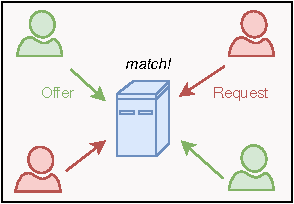
\includegraphics[width=.9\linewidth]{assets/centralized_matchmaking}
%		\caption{\emph{Centralized matchmaking}: new orders are always sent to a single matchmaker, usually a centralized system (server).}
%		\label{fig:centralized_matchmaking}
%	\end{subfigure}%
%	\begin{subfigure}[t]{.33\textwidth}
%		\centering
%		\captionsetup{width=.9\linewidth}
%		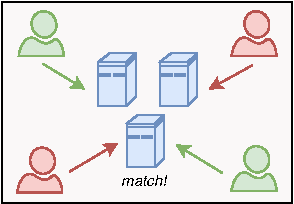
\includegraphics[width=.9\linewidth]{assets/federated_matchmaking}
%		\caption{\emph{Federated matchmaking}: new orders are sent to one of the available matchmakers in the network.}
%		\label{fig:federated_matchmaking}
%	\end{subfigure}%
%	\begin{subfigure}[t]{.33\textwidth}
%		\centering
%		\captionsetup{width=.9\linewidth}
%		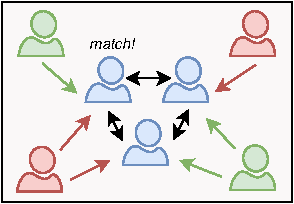
\includegraphics[width=.9\linewidth]{assets/decentralized_matchmaking}
%		\caption{\emph{Decentralized matchmaking} (our proposal): new orders are sent to multiple matchmakers and shared between them.}
%		\label{fig:decentralized_matchmaking}
%	\end{subfigure}
%	\caption{Three models for order matching. Traders create offers and requests (colored green and red respectively), which are matched by matchmakers (depicted in blue).}
%	\label{fig:matching_architectures}
%\end{figure*}

% Convince reviewers of the importance of matchmaking


%The main responsibility of many online service providers is to act as \emph{matchmaker} between their users.
%Acting as a trusted intermediary, or \emph{matchmaker}, between users is at the core of many online services providers.
%For example, the key objective of companies acting in the sharing economy, such as Airbnb (house sharing) and Uber (ride hailing), is to bring individuals together that can engage in an exchange of service or goods. %, is to act as trusted middleman for the services provided or requested by individual platform participants.
%Similarly, matching prospective traders with each other is a requirement for e-commerce platform operators such as eBay and Amazon.

%Online commerce platforms are pervasively used in both traditional and emerging markets. However, increasingly becoming critical infrastructure in our society, these platforms also bring systemic risks to everyday consumers~\cite{azevedo2016}\cite{oecd2019}.The full potential of these developments is hard to assess yet, but some key trends are already evident such as an unprecedented concentration of power by a few centralized intermediaries~\cite{pepper2019}.
%The operators of these platforms gain unprecedented power over market flows through the control of all the key enabling elements for marketplaces, including settlement, arbitrage, and matchmaking mechanisms.
%The latter element is of particular interest in this work as at the dawn of e-commerce matchmaking solutions were envisioned as key enabling elements for open and competitive ecosystems of marketplaces~\cite{trastour2002}.

%As a result, however, they increasingly become critical infrastructure in our society~\cite{oecd2019}\cite{azevedo2016} and, with raising influence of a few global players, a systemic risk to everyday consumers.
%However, as they increasingly become critical infrastructure in our society influenced by a few global platforms, it also brings systemic risks to everyday consumers ~\cite{oecd2019}\cite{azevedo2016}.

%Facilitating wide range of interactions between individuals and businesses on the global scale these platform intermediaries start to dominate both traditional and new markets~\cite{oecd2019}.

%The latter element is of particular interest in this work since matchmaking services built on the principles of semantic web became earlier building blocks of scalable e-commerce~\cite{trastour2002}. \todo{not clear how this sentence fits in logically. Why is it of particular interest? Because of semantic web? Because of early e-commerce - then why is it still relevant today?} 
%At the same time development of proprietary matchmaking solutions has significantly outpaced academic research in this area making it difficult to assess wider societal and economic impact
%Effective \emph{matchmaking} between users is an essential enabling component for electronic marketplaces.

%Matchmaking in electronic markets can be considered as the process of mediating between the supply and demand created by users~\cite{veit2002multi}.
%Furthermore, matchmaking can be seen as a universal element for the coordination of economic activity in general, ranging from the matching of asset suppliers to interested buyers, to the assignment of incoming workloads to idle computing resources.

%Currently, \emph{centralized matchmaking} is the approach taken by most commercial market operators~\cite{oecd2019}\cite{azevedo2016}.
%These operators deploy centralized matchmaking servers that are optimized to efficiently match new orders with the existing ones within a specific application domain, which has two main advantages.
%Firstly, the market operator can match incoming orders with the (current) best compatible order, since all orders are stored on their servers.
%Secondly, centralized matchmaking enables more simple software integration with other domain-specific services provided by the same market operator.

%Such opaque, algorithmic matchmaking mechanisms often can be exploited by market-operators to increase their intermediary revenues, through unfair match-making. These practices were identified through different e-comerce platforms [ref]. And the scale of this problem is highlighted by the current antitrust investigation into Amazon's suspected unfair treatment of customers by the European Commission~\cite{ec2019}. It has been also argued that these developments not only introduce unfair competition in e-commerce but can undermine the emerging sharing economy [ref].

%Emblematic of these issue are practices of Uber - operator of ride-hailing platform, implementing price discrimination and phantom matches to manipulate behaviour of its users [ref,ref]. It has been also demonstrated with experimental setups that Uber matchmaking algorithm undermines revenues of participants to the advantages of platforms operator[ref]. As researchers also point out this is a complex, multilayered issues that can not be mitigated only with adjustments in matchmaking algorithms[ref]. We suggest that this problem requires a radical re-thinking the role of trusted third parties as matchmakers. Decentralized matchmaking systems can be a first step towards mitigation of systemic risks stemming from the abuse of privileged intermediary position by market operators.

%Ineffective matchmaking by market operators not only decreases overall market efficiency and customer satisfaction, but also can result in price discrimination and unfair markets~\cite{Wu2015TheM} \cite{mikians2012}.
%For example, in a ride-hailing marketplace like Uber, it is key to match nearby drivers and passengers in a timely and efficient manner.
%For instance, suboptimal matching by ride-hailing marketplaces such as Uber can result in opaque price steering, and greater waiting time both for passengers and drivers~\cite{chen2015} \cite{azevedo2016}. 
%In fact, many of the electronic market operators usually deploy in-house, proprietary matchmaking solutions integrated with price personalization and recommender systems ~\cite{hannak2014}.\footnote{Recommender systems can also be used to enable 'price steering' - changing the order of search results for products and services.}

%Inefficient mediation by such matchmakers decreases the overall platform efficiency and user satisfaction~\cite{Wu2015TheM}.
%For instance, ride-hailing companies assign drivers to waiting passengers based on their geographical separation. % efficiently mediate between passengers, requesting transportation and drivers, willing to provide this service.
%Prolonged sub-optimal matching in this domain increases the waiting time for passengers and results in drivers having to traverse a greater distance to pick up their passengers.
%Equivalently, cloud services providers are tasked to ensure an efficient allocation of their computer resources to customers.
%Failing to do so could violate service-level agreements and result in customer loss and reputational damage.

%Users participate in the market by expressing their intentions in an \emph{order}, which is then submitted to the matchmaking server of the market operator.
%These \emph{centralized matchmaking} servers are optimized to efficiently match new orders with existing ones, within a specific application domain, which has two main advantages.\todo{cite}
%Firstly, the market operator can match incoming orders with the (current) best compatible order, since all orders are stored on their servers.
%Secondly, centralized matchmaking enables more simple software integration with other domain specific services provided by the same market operator.
%it is easier to implement the required software primitives when considering centralized matchmaking, compared to decentralized or distributed matchmaking models.

%For these reasons centralized matchmaking is the approach taken by the most commercial market operators.
%Unfortunately, due to the the proprietary nature of deployed matching algorithms they are specified and controlled by the market operator. 
%Unfortunately, many electronic markets deploy in-house, proprietary matchmaking solutions integrated with price personalization and recommender systems, fully specified and controlled by the market operator~\cite{hannak2014}.\footnote{Recommender systems can also be used to enable \enquote{price steering} by market operator - manipulating the order of search results for products and services in order to nudge users.}
%This raises up a question of contradictions between commercial interests of operators and the objectivity of chosen criteria for matchmaking efficiency~\cite{azevedo2016}.
%Ineffective matchmaking by market operators not only decreases overall market efficiency and customer satisfaction, but also can result in price discrimination and unfair markets~\cite{Wu2015TheM} \cite{mikians2012}.
%Thus, market operators have the capability to modify the matching algorithm so that it gives an (unfair) advantage to specific users \cite{mikians2012}\cite{azevedo2016}.
%Consequentially, the orders of a user might not be matched with the currently best compatible order, resulting in a system that is void of any transparency in the matchmaking process.
%In this model users have to rely on the trustworthiness of the market operator to conduct the matchmaking of their orders in a fair manner and not to engage in price discrimination or other manipulative practices.
%The scale of this problem is highlighted by the current antitrust investigation into Amazon's suspected unfair treatment of customers by the European Commission~\cite{ec2019}.
%The most recent and particularly disturbing illustration is the illegal gouging of prices on the products sold directly by Amazon itself in the heat of COVID-19 epidemic \cite{talmon2020}. 

%Specifically, this server iterates through all existing orders to find matches, based on a matching policy.
%Even though most market operators follow this approach, we identify three deficiencies:
%\begin{itemize}
%	\item \textbf{Unfairness}: 
%Since the matching algorithm is usually not open for inspection by traders, the broker is allowed to match according to their own rules, e.g., to maximize commission fees or to prioritize specific users.

%\item \textbf{Low resistance against large-scale failures}: even though major electronic marketplaces take measure to detect and prevent infrastructure failures, centralized architectures are not resistant against certain events that affect the infrastructure as a whole, e.g., misconfiguration, DNS issues or DDos attacks.
%If the matchmaking infrastructure becomes unavailable, new orders cannot be processed and all market activity stalls.
%\item \textbf{Lack of re-usability}: Due to competitive motivation, the specifications of deployed matchmaking infrastructure and algorithms are often proprietary, and highly domain-specific.
%Therefore, these solutions are not re-usable by other market operators, potentially providing similar services.
%As a result, there exists a large range of non-compatible infrastructure for matchmaking in electronic markets.
%\end{itemize}

%The necessity of a trusted centralized market operator has been challenged by the advancements in decentralized technologies such as blockchain.
%Advancements in decentralized technologies, e.g., blockchain technology, have questioned the role of trusted intermediaries.
%Blockchain technology provides the means to manage a distributed ledger on which users can securely transfer value (e.g., Bitcoin~\cite{nakamoto2019bitcoin}) or deploy decentralized applications (e.g., Ethereum~\cite{wood2014ethereum}) without explicit approval from a trusted third party.
%Decentralized exchanges (DEXes) operating on the basis of blockchain facilitate the trade of digital assets or services without the requirement for a market operator~\cite{subramanian2017decentralized}.
% have resulted in a new type of electronic market: blockchain-based exchanges, or DEXes.
%The problem of efficient matchmaking is re-visited with the deployment of decentralized exchanges based on blockchain technology, also called DEXes.
%These exchanges, also called DEXes, enable traders to securely trade cryptocurrencies and digital assets without a central market operator.
%No trusted third party is needed for the exchange of value, unlike most existing electronic marketplaces.
%In contrast to existing electronic marketplaces, markets powered by blockchain technology, also called DEXes, enable traders to securely exchange digital tokens without a trusted third party.
%The existing research on DEXes addresses the question on \emph{how} to securely exchange value between users, but deems order matchmaking as uninteresting or out of scope~\cite{daian2019}.
%Some DEXes provide one or more matchmaking servers that process market orders~\cite{eskandari2019} ~\cite{idex}\cite{warren20170x}.
%In practice, however, these approaches rely on a few or a single server and therefore still carries limitations on the achievable level of fairness and transparency desirable on such markets.
%Alternatively, the (on-chain) deployment of order matchmaking algorithms on a blockchain addresses the issue of transparency.
%Yet, scalability issues inherent to all the blockchain protocols based on a global consensus carry significant limitations on the speed at which matchmaking can be conducted (also see Section~\ref{sec:experiments_ethereum})~\cite{daian2019}.
%Apart from that, such on-chain implementations based on smart contracts where time and order of transaction execution is critical, demonstrate vulnerability to \emph{transaction re-ordering} and \emph{front-running} attacks ~\cite{eskandari2019}\cite{kolluri2018}\cite{judmayer2019}.
%These contradictions effectively create a dilemma of choice between two desirable properties of matchmaking mechanisms.
%Efficiency of matchmaking achievable through the concentration of orders by a trusted central party, versus provable fairness of matchmaking achievable with the transparency of decentralized on-chain matchmaking.
%We argue, however, that these contradictions do not present an insurmountable obstacle for the implementation of efficient and fair matchmaking solutions. \todo{Georgy (I commented out the contributions)}

%is often performed by a centralized server that collects buy and sell orders, and match them. 
%This centralized approach, however, stands in stark contrast to the decentralized ecosystems that blockchain technology enables.
%Other solutions embed the matchmaking algorithm in the transaction validation process and essentially perform matching on the blockchain (\enquote{on-chain}).
%Unfortunately, this approach is vulnerable to the front-running attack where a specific validator can ultimately decide how specific orders are matched.
%As the number of services for decentralized finance (DeFi) and trade proliferates, there is a growing need for a reliable and re-usable matchmaking mechanism that matches orders in a fair and reliable manner, without centralized control and usable across different domains.
%There currently is no such mechanism available.

%Order matchmaking in various DEXes is a centralized process and performed by a dedicated entity. %/, which is against the decentralized nature of a blockchain ledger.
%Besides aforementioned issues, we argue that centralized matchmaking contradicts the decentralized nature of blockchain ledgers.
%Newer DEX architectures allow for multiple, independent matchmakers that each maintains a list of all current offers and requests~\cite{warren20170x}.
%Traders then submit new orders to one of the available matchmakers.
%New orders created by traders are are matched with others and the exchange of assets then proceeds on the blockchain ledger.

%Within the field of distributed systems, matchmaking is highly related to Publish/Subscribe (pub/sub) architectures\footnote{Some literature in distributed systems refers to an intermediating peer as a \emph{broker}. We use the term matchmaker since we determined it to be more commonly used in related work.}.\todo{rewrite}
%Order brokering is strongly related to Publish/Subscribe (pub/sub) architectures where subscribers indicate their interest in notifications and publishers disseminate new events.
%The main issue is to devise decentralized broker architectures to mediate between publishers and subscribers.
%One might argue that a decentralized pub/sub architecture is sufficient to 
%However, order brokering is a process where the state of individual orders should be updated when successfully matched with other orders, whereas events and notifications in pub/sub systems are static pieces of information.
%Even though there is a substantial body of work on matchmaking in distributed systems, there is no work that researches the properties of decentralized matchmaking in the context of orders.

%Matchmaker is a key concept in Publish/Subscribe (pub/sub) architectures, where one or more brokers deliver events, generated by publishers, to interested subscribers\footnote{Some literature in distributed systems refers to an intermediating peer as a \emph{broker}. We use the term matchmaker since we determined it to be more commonly used in related work.}.
%One might consider an distributed pub/sub architecture where order creators are considered publishers and subscribers are interested in fulfilling specific orders.
%The main issue with this approach is 

%Even though there are many efforts to enable secure value transfer between users without requirement for a trusted broker, there is a lack of understanding \emph{how} these users can connected.
%For this reason, many 

%Matchmaking is defined as the process of mediating supply and demand in markets~\cite{veit2002multi}.

%Notable examples are matching idle agents to incoming jobs or matching suppliers of specific assets to consumers who are interested in buying these assets.

%For example, in a ride-hailing marketplace like Uber, it is key to match nearby drivers and passengers in a timely and efficient manner.
%For instance, prolonged suboptimal matching by ride-hailing marketplaces such as Uber increases the waiting time for passengers and results in drivers having to traverse a greater distance to pick up their customers.


%Traditionally, this is performed by a centralized entity.

%\textbf{Contributions.}
%We present \emph{MATCH}, a decentralized middleware for fair order matchmaking, based on the principle of strictly decoupling the matching process from the negotiation of trade agreements. We evaluate MATCH using two workloads for ride-hailing and asset trading, reconstructed from real world traces. We consider ride-hailing as a paradigmatic case to demonstrate fair decentralized mechanisms for matchmaking. Unlike the centralized matchmaking mechanism where orders can be prioritized, hidden, or delayed by a market operator, MATCH provides fair matching for counter-parties who then engage in a peer-to-peer negotiation process with prospective trading partners.

%Furthermore, with asset trading experiment we show that MATCH does not rely on the specifications of orders, and is therefore re-usable across different trading domains. Our experiments demonstrate that MATCH exhibits excellent resistance against selfish matchmakers attempting manipulate matches, while establishing matches with high quality. Furthermore, we show that MATCH has memory, bandwidth usage, and order fulfill latency that are several orders of magnitude lower compared to matchmaking on an Ethereum blockchain.

%Our main contribution is the MATCH protocol itself where any user can act as a matchmaker for others.
%Matchmakers store open orders created by users, matches incoming orders with existing ones, and inform order creators about potential matches.
%And, since users themselves are ultimately responsible for deciding who they will negotiate with, MATCH exhibits resistance against matchmakers which deviate from an agreed matching algorithm. 
%Order creators disseminate a new order to multiple matchmakers while avoiding network-wide replication of orders. 

%The contribution of this work can be summarized as follows.
%Our first contribution is the MATCH \emph{protocol} where any user can act as a \emph{matchmaker} for others.
%Matchmakers store open orders created by users, matches incoming orders with existing ones, and inform order creators about potential matches.
%Unlike deployed centralized approaches, the role of matchmakers is to \emph{notify} order creators about matching orders and potential counterparties; users then contact these potential counterparties and engage in a peer-to-peer negotiation process.
%Unlike the centralized matchmaking mechanism where orders can be prioritized, hidden, or delayed by a market operator, MATCH provides fair matching for counter-parties who then engage in a peer-to-peer negotiation process with prospective trading partners.
%And, since users themselves are ultimately responsible for deciding who they will negotiate with, MATCH exhibits resistance against matchmakers which deviate from an agreed matching algorithm.
%Order creators disseminate a new order to multiple matchmakers while avoiding network-wide replication of orders.

%The second contribution is the MATCH middleware for fair order matchmaking.
%MATCH does not rely on the specifications of orders, and is therefore re-usable across different trading domains.
%We evaluate MATCH using two workloads for ride-hailing and asset trading, reconstructed from real-world traces.
%Our experiments demonstrate that MATCH exhibits excellent resistance against matchmakers that pursue selfish interests, while establishing matches with high quality.
%Furthermore, we show that MATCH has memory, bandwidth usage, and order fulfill latency that are several orders of magnitude lower compared to matchmaking on an Ethereum blockchain.
%First, in comparison to centralized exchanges, MATCH provides traders with an environment in which that is  \emph{fairness}.
%Second, MATCH is designed around \emph{reliability} and can deal with crash failures of individual brokers.
%Finally, MATCH is \emph{reusable} across different domains that require brokering of homogeneous orders, e.g., the sharing economy, peer-to-peer energy trading and decentralized cryptocurrency exchanges.



%\todo{key insights}

%The main contribution of this work is two-fold.
%Our first contribution is the design of a novel, decentralized order matching protocol.

%Our first contribution is the MATCH middleware, for fair and reliable order brokering in different decentralized environments.
%The second contribution is the MATCH middleware for generic order matching and an accompanying implementation in the Python programming language.

%We identify two problems of existing centralized approaches to matchmaking engines:
%\begin{itemize}
%	\item \textbf{Transparency - } TODO
%	\item \textbf{Unfairness - } TODO
%	\item \textbf{Fault Tolerance - } TODO
%\end{itemize}

%Within the context of distributed systems, there have been efforts to ... \todo{semantic matchmaking}

% The order book 

%Automatically \emph{matching} customers is essential for electronic marketplaces.
%More generally, matchmaking is defined as the process of mediating supply and demand in markets~\cite{veit2002multi}.
%Notable examples are matching idle agents to incoming jobs or matching suppliers of specific assets to consumers who are interested in buying these assets.
%Inefficient matchmaking between participants decreases overall market efficiency and customer satisfaction~\cite{Wu2015TheM}.
%For example, in a ride-hailing marketplace like Uber, it is key to match nearby drivers and passengers in a timely and efficient manner.
%For instance, prolonged suboptimal matching by ride-hailing marketplaces such as Uber increases the waiting time for passengers and results in drivers having to traverse a greater distance to pick up their customers.

%It is common practice for market providers to offer centralized infrastructure that automatically matches new incoming orders with existing ones. %and accepts incoming orders and matches them with other others.
%More specifically, platform participants submit orders to a centralized server.
%This server then attempts to find a match with other orders that are active in the market.
% each company has their own locked-in matching logic.
%All active orders are bundled in an \emph{order book}.
%This data structure keeps track of all market orders that have been submitted by traders.
%New orders, are inserted in the order book and matched against existing entries.
%These servers keep track of the full order book which contains the current list of all active buy and sell orders created by platform participants.
%Centralized matchmaking is deployed by many commercial marketplaces such as Uber, Airbnb and Nasdaq.
%Although this centralized approach to matchmaking is adopted by a vast majority of electronic marketplaces, it leads to a few deficiencies.
%First, centralized order matchmaking architectures tend to be less resistant against infrastructure failures and targeted attacks (e.g., a denial-of-service attack~\cite{mirkovic2004internet}).
%Second, the deployed matching logic is rarely open for inspection by traders and therefore prone to manipulation by market operators.
%For example, Uber has actively manipulated the matching algorithm between drivers and passengers, based on ride pricing~\cite{chen2015peeking}.

%To improve fault tolerance and scalability, the effectiveness of using multiple, independent matchmaking entities has been explored.
%This model, also called \emph{federated matchmaking}, is presented in Figure \ref{fig:federated_matchmaking}.
%The key idea is that each matchmaker takes responsibility for managing a part of the global order book.
%In federated matchmaking architectures, matchmakers often operate highly isolated from each other and do not synchronize orders with each other.
%This isolation potentially leads to missing better matches.

%While numerous electronic marketplaces have deployed (proprietary) matchmaking logic, there is no generic architecture for order matching that is re-usable within different trading domains.
%This results in incompatible applications, all with custom architectural decisions and assumptions regarding workload and environment. % optimized to  under certain assumptions, environments and workloads.
%We address this shortcoming and present MATCH: a middleware for generic order matching.
%Since MATCH does not make any assumptions on the specifications of orders, our middleware i. % and does not make any assumptions on the details of orders being matched.
%This work first outlines two existing models for order matchmaking (Section \ref{sec:background_problem_description}).
%Based on fundamental deficiencies of existing matchmaking approaches, we introduce a new model: \emph{decentralized matchmaking}.
%Next, we present the MATCH protocol, architecture and implementation (Section \ref{sec:protocol}, \ref{sec:architecture} and \ref{sec:implementation}).
%MATCH is designed around the decentralized matchmaking paradigm, yet has full compatibility with existing approaches for order matchmaking. %, while maintaining compatibility with traditional models.
%Finally, we evaluate the performance of MATCH with a ride-hailing and asset trading workload, reconstructed from real-world datasets (Section \ref{sec:experiments}). %, and then design a novel architecture and protocol for decentralized matching of orders.
%This results in an architecture and protocol with high fault tolerance and scalability.

%A major issue is that the matching of two orders by \enquote{consumes} these resources and subsequently should be removed from the order books maintained by brokers.

%In this work, we address the challenging task of devising a network where individual order brokers maintain a decentralized order book.
%These brokers, however, might have adversarial intentions and actively attempt to influence the matchmaking protocol to their own benefits.
%We argue that the availability of such an order book 
%To the best of our knowledge, we are the first to explore order brokering from the context of decentralized markets.

%\newpage

\begin{figure}[t]
	\centering
	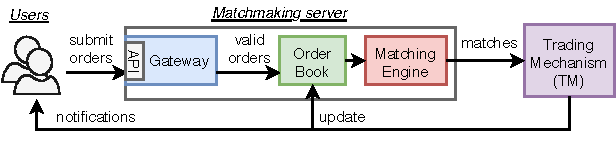
\includegraphics[width=\linewidth]{match/assets/central_exchange_architecture}
	\caption{A generic model for centralized matchmaking in peer-to-peer markets, using a single matchmaking server.}
	\label{fig:central_exchange_architecture}
\end{figure}

\section{Towards Decentralized Matchmaking}
\label{sec:centralized_order_matchmaking}
In our approach, users in a peer-to-peer market conduct the matchmaking process themselves.
To elaborate on the components used in our solution, we first devise a generic, centralized model for matchmaking.
We then identify technical concerns that arise when decentralizing this model.

\subsection{Centralized Matchmaking}
We devise a generic model for centralized matchmaking in peer-to-peer markets, see Figure~\ref{fig:central_exchange_architecture}.
This model is the starting point for our fair matchmaking solution and is inspired by existing architectures that have been widely used by financial markets~\cite{mavroudis2019libra,veit2003matchmaking}.
Users create \emph{orders}, which they then submit to the matchmaking server.
An order specifies interest to buy or sell assets, resources, or services (orders are further discussed in Section~\ref{sec:order_creation}).
Many markets deploy one or more gateways that filter out invalid orders and mitigate targeted attacks on the matchmaking server, such as a DDoS attack~\cite{mavroudis2019libra}.
Valid orders are inserted in the \emph{order book}, a local data structure that bundles all open and valid orders.

Upon the insertion of a new order in the order book, it is forwarded to the \emph{matching engine}.
This component searches for existing orders in the order book that match with the newly submitted order.
In particular, an incoming order should be matched with the current best compatible order(s).
Whether two orders match is predicated by a \emph{matching policy}.
For example, the price-time strategy is a predominant matching policy in financial markets where orders are first matched based on their price and then on their creation time (prioritizing older orders)~\cite{mavroudis2019libra}.
The matching engine can establish multiple matches for a single order, e.g., a buy order for a large number of assets can be matched with multiple (smaller) sell orders.
Established matches should be \enquote{executed}, which is an application-dependent operation.
In a financial exchange, for example, the specified assets in the matched orders should be exchanged between the order creators.
In a ride-hailing market, however, the driver and passenger should be put in contact with each other.
We model the component that executes established matches as the \emph{trading mechanism} (TM), which we consider external to the model in Figure~\ref{fig:central_exchange_architecture}.
After established matches have been executed by the TM, the affected orders in the order book are updated (or removed if they are completed), and the order creators are notified of the match execution.
%Upon receiving a notification from the trading mechanism, the order creator internally updates the state of their affected order.
%We assume that the TM executes matches in a first-come-first-serve manner.
%After a match has been executed, the matched orders in the order book are updated (or removed if the order is completed), and the order creators are notified about this event.
%This unit \enquote{executes} the established matches and ensures that the creators behind these orders trade the services as specified.
%The matching engine forwards established matches to the MPU, updates the matched orders in the order book accordingly, and notifies the user(s) behind the matched orders of the event. % The current state of the order book is updated and matched orders that are completed are removed.
%The order creators are then notified about the updated state of their order.
%A matchmaker bundles open orders in a local data structure known as an \emph{order book}.
%This order book is often optimized for fast order lookup and matching within a specific trading domain.
% to achieve load balancing and protection against 

%Figure~\ref{fig:central_exchange_architecture} illustrates the data flow when submitting a new order to a centralized order broker.\todo{explain}

%Figure~\ref{fig:centralized_matchmaking} visualizes the centralized matchmaking model, which is the most common approach to match orders.
%The most common model for order matchmaking uses a centralized approach to match platform participants, see Figure \ref{fig:centralized_matchmaking}.
%Traders send new offers and requests to a dedicated matchmaker, usually a centralized system (server).
%This model is widely adopted by commercialized marketplaces such as stock exchanges or peer-to-peer service markets like Uber.
%This matchmaker listens for new orders and matches incoming orders them with existing orders in the market.

\subsection{Decentralized Matchmaking}
\label{sec:towards_fair_reliable_matchmaking}
The model in Figure~\ref{fig:central_exchange_architecture} allows the server operator to conduct unfair matchmaking by manipulating the matching engine (or policy) to hide, prioritize, or delay specific orders.
To address this situation, we propose a solution where users (order creators) themselves carry out matchmaking while ensuring that no single user can authoritatively decide on how the orders of other users are executed.
We first consider a basic, decentralized architecture where every user operates a single matchmaking server.
A user then submits a new order to all matchmaking servers, and all servers forward established matches to the same TM.
The TM executes incoming matches in a FCFS manner.
%If an adversary now manipulates a strict subset of matchmaking servers, the TM would still be able to execute the best match for an order among all found matches by simply aggregating the incoming matches for a specific order during some time.
%If there is at least one honest matchmaker that has established the current best match for a specific order, the TM should execute this match, therefore nullifying the impact of the manipulation.
This approach, however, raises the following technical concerns:

\emph{1) How does a decentralized matchmaking architecture process matches of the same order found by distinct matchmaking servers?}
Deploying a single matchmaking server prevents the situation where distinct matchmaking servers submit the same or different (valid) matches for the same order to the TM.
Assuming a FCFS execution of incoming matches by the TM, having multiple matchmaking servers sending matches to the TM likely results in the situation where matches of the same order are executed multiple times, resulting in an incorrect order state.
To ensure correctness, our replicated matchmaking architecture requires additional coordination. % to avoid that the same match is executed multiple times.

One solution involves the periodic execution of a Byzantine fault tolerant consensus protocol by matchmaking servers to decide which matches are sent to the TM.
Unfortunately, reaching consensus is a resource-intensive process and existing protocols, e.g., PBFT~\cite{castro1999practical} or Proof-of-Work~\cite{gervais2016security}, do not scale when the number of matchmaking servers or orders increases~\cite{vukolic2015quest}.
We avoid the need for consensus by having users \emph{negotiate} trade agreements with potential counterparties (further described in Section~\ref{sec:order_negotiation}).
Upon a positive negotiation outcome, these trade agreements, digitally signed by both parties, are sent to the TM and executed.
Matchmakers only \emph{notify} users about potential matches for their orders.
Since it is in the best interest of users to correctly manage their orders, rational users will not sign trade agreements that would result in an incorrect order state.

%Users then initiate negotiation with potential trade counterparties (further described in Section~\ref{sec:order_negotiation}).
%Upon reaching a trade agreement, both parties forward this agreement to the TM.
%The TM executes incoming trade agreements.
%Negotiating parties submit the negotiation outcome to the TM if they reached a trade agreement, which is then executed.

\emph{2) Is it required to disseminate a new order to all matchmaking servers?}
In the architecture described above, a user sends a new order to all matchmaking servers.
This results in full replication of the order book, under the assumption that all matchmaking servers eventually receive every new order.
The problem is that a flooding-based dissemination strategy leads to severe performance degradation when the number of matchmaking servers increases, as illustrated by deployed peer-to-peer applications like Gnutella~\cite{chawathe2003making}.
We address this concern by sending a new order to a small, random subset of all matchmaking servers such that it is still likely that at least one honest matchmaking server receives compatible orders (further described in Section~\ref{sec:order_dissemination}).

%If we assume that the MPU processes orders in a first-come-first-serve manner, matchmakers with a malicious intent can attempt to be the first to submit a sub-optimal match for some order to the MPU.\todo{relate to on-chain matching}
%As an alternative, the MPU can collect multiple incoming matches and after some timeout, make a selection on which matches to execute.
%This approach, however, would require the MPU to run matchmaking logic 
%With this approach, however, the MPU resembles a centralized server that serializes incoming matches, and ignore invalid ones.

%In the replicated matchmaker architecture, matchmakers with malicious intent could match incoming orders according to their own matching logic and submit sub-optimal matches to the MPU.
%If the MPU would process matches in a FCFS order, it could accepts a sub-optimal match from a broker with low latency to the MPU.
%Furthermore, the MPU should not execute the same incoming match twice.\todo{relate to blockchain matching}
%\item \emph{How can we prevent that sub-optimal matches established by a malicious broker are accepted by the match processor?}

%In the remainder of this work, we further elaborate on our solution for fair order matchmaking, named \emph{MATCH}.

%We consider an architecture where the brokering functionality is replicated over $ n $ potentially adversarial entities in the network.
%Traders disseminate new orders to all $ n $ brokers in the network.
% what if a malicious broker is the first to submit a malicious order to the order processing engine?

%Given the deficiencies of centralized matchmaking, and the issues when replicating the matchmaker functionality, we formulate the overarching research question of this work as follows: \emph{how can we build a re-usable, decentralized middleware for fair and reliable order brokering, suitable to be deployed on the Internet?}

\section{System and Threat Model}
We address the aforementioned concerns and present a decentralized middleware for fair matchmaking, named \emph{MATCH}.
We now outline the system and threat model of MATCH.
%In this work, we specifically focus on resistance against matchmakers that pursue selfish interests.
%The aim of MATCH is not to find a Pareto-efficient matching, which is not how most electronic markets operate.
%This model is predominant choice of most electronic marketplaces.
%If incentives are required, the MPU can award the matchmakers upon finding a successful match.
%The threat model focusses on  fairness and reliability.
% Does not need to work for millions! What's a reasonable network size?
%\subsection{System Model}
%We first provide a system model that specifies the market and order model, actors, and assumptions on the network.

\textbf{Market and order model.}
%Matchmaking depends on the individual constraints and preferences of market participants.
%In most electronic markets, a participant includes this information in an \emph{order} that indicates their intention to buy and sell assets, resources, or services~\cite{veit2003matchmaking}.
%This order is then submitted to a broker.
%Each order can have multiple attributes attached, e.g., a price or a location.
%The main objective of a broker is a quick and effective mediation between incoming offers and requests.
We adopt a continuous market model where orders are matched in a FCFS manner.
This model is commonly used by peer-to-peer markets (e.g., by Uber).
To represent a two-sided market with supply and demand, we introduce two order types: \emph{offers} and \emph{requests}.
Offers, respectively requests, indicate interest to sell, respectively buy specific assets, services, or resources.
%Besides a few required fields (see Section~\ref{sec:order_creation}), the order specification is not fixed.
To ensure re-usability across different markets, matchmakers in MATCH can host multiple order books and manage orders with differing specifications.
Each order has a quantity $ q $, which is an integer value indicating the number of assets, services, or resources being offered or requested.
The state of an order can be either \emph{open} (when the order has a positive quantity, $ q > 0 $), \emph{completed} (when all quantity in the order has been traded, $ q = 0 $), \emph{cancelled} (when the order has been cancelled by its creator) or \emph{expired} (when the timeout of the order has expired).
The structure and content of an order are further elaborated in Section~\ref{sec:order_creation}.
%Offers and requests of the same type are stored in the same order book.
%Many electronic markets exclusively process homogeneous assets, services or resources that can be expressed with a fixed number of attributes.
%Therefore, we limit the expressiveness of orders in this work such that it considers only homogeneous items.
%Offers and requests specify the interest in or availability of homogeneous items.
%These orders can be expressed with a fixed number of attributes, and can be compared with each other without much computational overhead.
%In contrast, heterogeneous products possibly have many attributes and constraints and often expressed used an ontology.
%For instance, information in semantic matchmaking is often represented using an ontology with support for multi-dimensional attributes and rich metadata.
%.  % \todo{we limit to one-dimensional matchmaking}

\textbf{Actors.}
We refer to an entity in the MATCH network as a \emph{node}.
A node can act as a \emph{user}, \emph{matchmaker}, or take on both roles.
Users disseminate offers and requests to matchmakers.
MATCH requires the active participation of users to negotiate with other users and thus requires users to be online for their order to be completed (also see Section~\ref{sec:order_negotiation}).
%Matchmakers store incoming orders from users in their order books and attempt to match them with exiting ones.
%This incentive could further be improved further by introducing monetary incentives such as transaction fees, which is outside the scope of this work.
%MATCH requires users to remain online while their order is not completed. %, and to ensure availability when negotiate a trade with matched parties.
%Since users have an incentive to complete their order, we believe this is a reasonable requirement.
%A matchmaker aggregates market orders and therefore has knowledge that can be utilized when creating new orders.
%This is an incentive to act as matchmaker.

%Alternatively, one might design a protocol without dedicated matchmakers where a trader queries other traders to find potential trading partners (for example, by performing an exhaustive search).
%Since the maximum number of queries one has to perform then directly grows with the network population, this is not a scalable approach.
%Also, MATCH is not designed to find a Pareto-efficient (stable) matching set since this would require an offline algorithm where all orders are created before the matching algorithm starts~\cite{Brito2005DistributedSM}.
%This is infeasible in markets with a continuous, dynamic arrival of new orders.
%Instead, we use an opportunistic approach where matchmakers immediately attempt to match incoming offers and requests.

%The MATCH protocol handles the unavailability of traders, is asynchronous and does not require clock synchronization.
%The three protocol phases are now explained in more detail.
%In comparison to this work, their protocols are designed around a specific use case.

\textbf{Network.}
We aim for MATCH to be deployed in a WAN environment.
We consider an unstructured peer-to-peer network where each node knows the network addresses of active matchmakers.
This can be achieved by maintaining a list of matchmakers, e.g., on a website or through a decentralized publishing network like the Kademlia DHT~\cite{maymounkov2002kademlia}.
New matchmakers enrol themselves on this list while matchmakers leaving the network un-enrol from this list.
As we show in Section~\ref{sec:order_dissemination}, MATCH is able to deal with offline matchmakers that are still enrolled on the list.
Users periodically download the latest version of this list to keep up with the set of active matchmakers in MATCH.
%Users periodically synchronize their local copy of this list with the latest published version.

%Each peer in the network can act as a user, matchmaker, or both.
Each node possesses a public and private key.
The public key is used to identify the node in the network whereas the private key is used to sign all outgoing network messages.
%Messages between nodes are authenticated.
We assume that the digital identity of each node in MATCH is tied to a real-world identity, preventing uncontrolled identity creation (also known as the Sybil Attack)~\cite{douceur2002sybil}.
%Identity validation should be performed by a Registration Authority (RA) which is external to our system.
This is not an unrealistic requirement since many electronic marketplaces already impose identity verification in order to participate~\cite{damiani2003managing}.
Identity verification can, for example, be achieved by using the services of a centralized registration authority.
We note, however, that a centralized dependency might be undesirable in marketplaces with a decentralized structure.
In such marketplaces, we encourage the use of (semi-)decentralised solutions for identity management, like self-sovereign identities~\cite{muhle2018survey,stokkink2020truly}.

\textbf{Threat Model.}
\label{sec:threat_model}
In this work, our threat model orients around \emph{malicious matchmakers} that deviate from a standard matching policy and match incoming orders according to a custom policy.
For example, a matchmaker can deliberately match an incoming offer with the second-best request in their order book and match one of their own offers with the hidden request instead.
This threat model also captures collusion, the situation where a subset of matchmakers agrees to match orders according to a custom policy to gain economic benefit as a group.
Malicious matchmakers are often driven by economic incentives, e.g., when a matchmaker wants to prioritize its own orders or when a group of matchmakers collectively attempt to drive competitors out of business by ignoring their orders.
Malicious matchmakers directly affect market fairness since they treat incoming orders unequally.
We assume that cryptographic protocols are secure and that the computational power of adversaries is bounded.
%Specifically, an individual broker is able to deploy a custom matching policy which differs from the expected policy.
%One cannot distinguish a peer that went offline or a peer that deliberately refuses to respond to incoming messages.
%The MATCH protocol must take the presence of such peers into account.\todo{rewrite}
%This also means that any broker can decide to e incoming orders and not process then further, essentially censoring the orders created by specific peers.
%This is indistinguishable from the situation where a benign broker has crashed.

%By a real-world evaluation with a realistic ride-hailing and asset trading workload, we show that our middleware shows desired system properties, like accuracy, fault-tolerance and resistance against malicious matchmakers.

%in this architecture, participants can either voluntarily act as matchmaker for others or a committee of matchmakers is assembled.
%Each individual matchmaker maintains and acts on their own order book.
%Federated matchmaking has been evaluated by prior research work in the context of distributed resource allocation, where incoming jobs should be allocated to idle computer resources.
%More recently, this matchmaking approach is implemented by blockchain-based marketplaces such as 0x and ? that maintain an order book off-chain.
%In their approaches, matchmakers operate highly isolated from each other and there is no synchronization of order data amongst them.
%This results in order book fragmentation and potentially leads to missing better matches.
% divided on geographical properties... ?

%A platform participant sends their buy and sell orders to a single matchmaker.
%Each matchmaker maintains their own order book which does not necessarily contain a snapshot of all active buy and sell orders in the network.
%In this architecture, matchmakers do not share order information with other matchmakers.
%Matchmaker enrollment usually is an unpermissioned process that does not require approval.
%Federated matchmaking has been used to address the problem of distributed resource allocation, which goal is to allocate jobs to idle computer resources in a distributed fashion.
%Recent blockchain-based marketplaces also adopt this model to store and match orders.

% motivated by...

%In this work, we present MATCH, a decentralized, generic and scalable order matching middleware.
%Its distinguishing property is that order information is actively shared between matchmakers, see Figure \ref{fig:decentralized_matchmaking}.
%We design, implement and evaluate a generic middleware for order matching.
%Unlike much related work, we do not resolve our design around a class of orders with specific properties.
%This makes our middleware highly applicable across different domains, as we will demonstrate by an experimental evaluation with different workloads.
%Our work is motivated by the lack of scientific evaluation of fully decentralized and generic matchmaking architectures.
%The goal our work is to expand our knowledge of decentralized matchmaking architectures under changing network circumstances and in different trading situations.
%We particularly focus on fundamental distributed systems properties of our matchmaking middleware.
%An evaluation from an economics perspective can be found in related work~\cite{chan1998information}.

%In this work, we focus on \emph{decentralized matchmaking}, depicted in Figure X.
%The key difference between federated and decentralized matchmaking is that order information is shared between matchmakers in the latter model.
%The distinguishing property of this architecture is that matchmakers actively share order book information with each other.
%New buy and sell orders are disseminated in the network and matched by \emph{any} interested matchmaker.
%We are the first to perform a systematic evaluation of the performance of full decentralized matchmaking, to the best knowledge of the authors.
%Concretely, we design, implement and evaluate an order matching middleware which is highly generic and can be adopted in many market contexts.
%Our middleware resides between a peer-to-peer network and a trading mechanism.
%Unlike much related work, we do not make assumptions on the type of resources, goods or services being exchanged between participants.




% introduce architectures

%Numerous marketplaces like Uber, Airbnb and Nasdaq have to process and match thousands of new buy or sell requests every second.\todo{cite}
%Such marketplaces have deployed one or several servers which keep track of all incoming buy and sell orders. % which is fully owned and controlled by the market operator.
%This centralized method of matchmaking is shown in Figure X, where buyers and sellers directly submit new (buy or sell) orders to their matchmaker servers.
%However, centralized matchmaking leads to a few deficiencies in general.
%Centralized architectures tend to be less resistant against infrastructure failures and targeted attacks (e.g., a denial-of-service attack~\cite{mirkovic2004internet}).
%Second, the deployed matching logic of (commercial) market operators is rarely open for inspection by traders.
%This motivates market owners to exploit their prominent position.
%For example, it is suspected that Uber manipulates ride prices with their dynamic pricing mechanism (surge pricing)~\cite{chen2015peeking}.

%In recent years, much effort is spent on the design and deployment of decentralized blockchain-based exchanges, also called DEXes.
%The idea of DEXes is that order creation, matching and trade proceeds entirely on a distributed ledger (\emph{on-chain}).
%The first generation of DEXes either integrate matchmaking logic directly in the blockchain layer (BitShares) or deploy centralized matchmaking servers (IDEX).

%While DEXes allow for secure trading, it is inefficient to store the entire set of orders on the blockchain itself.
%Since each transaction requires a small fee to be paid by their issuer, trading on a DEX can be a costly process, especially since cancellation of orders also requires such fees.
%Second, there can be a considerable latency between submitting a new order and inclusion of this order on the blockchain ledger.

%More recent DEX architectures like 0x decouple storage of the order book and actual asset exchange.
%These architectures adopt a \emph{federated matchmaking} model where a few entities are in charge of matching .
%In this architecture, a trader selects a single matchmaker entity and submits their order to this entity.
%There is however no communication among these matchmaking entities, which may result in missing better matches and decreased market efficiency.

%In this work, we design and build a fully decentralized order matching mechanism, called MATCH.
%The design of MATCH is guided by identified issues with centralized and federated matchmaking policies.
%By rigorous scientific experiments, we explore key properties like scalability, fault-tolerance and efficiency of MATCH.
%MATCH is particularly useful in the presence of multiple types of order books, e.g. for cryptocurrency exchanges.
%We show how our middleware behaves when exposed to different workloads like stock trading and ride-hailing.

%\section{Background and Problem Formulation}
%\label{sec:background_problem_description}

%Automated order matching is an essential feature of many electronic marketplaces.
%We elaborate on existing approaches, used by academia and industry.
%Next, we formulate the main research question of this work.

%\subsection{Models for Order Matchmaking}
%\label{sec:matchmaking_models}

%\textbf{Federated matchmaking} - 
%Figure \ref{fig:federated_matchmaking} illustrates an alternative model for order matching: federated matchmaking.
%Instead of relying on a central matchmaker, multiple (independent) matchmakers individually maintain an order book.
%The group of matchmakers can either be static (e.g., elected by a committee or a voting mechanism), or dynamic (e.g., each peer can opt-in to become a matchmaker).
%A trader now submits new orders to their preferred matchmaker (for example, based on the reliability or trustworthiness of individual matchmakers).
%Blockchain-powered marketplaces based on the 0x and AirSwap protocols have adopted the federated matchmaking model~\cite{warren20170x}~\cite{swap}.
%This model has also been used in the context of resource allocation, where free computer resources are matched to incoming jobs~\cite{ebrahimi2004matchmaking}.
%Unavailability of an individual matchmaker is less likely to stall market activity since a trader can send their orders to another available matchmaker.
%However, matching effectiveness is lower since orders are fragmented across multiple matchmakers.

%\textbf{Decentralized matchmaking} - 
%Scalability limitations, low fault tolerance, and uneven load balancing are inherent issues of centralized and federated matchmaking.
%We propose the \emph{decentralized matchmaking} model, depicted in Figure \ref{fig:decentralized_matchmaking}.
%The main idea is that a single order is sent to multiple matchmakers simultaneously and matchmakers share their orders with other matchmakers.
%We identify two advantages of this model over centralized and federated matchmaking.
%First, sharing orders between matchmakers can yield the same matching effectiveness compared to centralized matchmaking, depending on the order synchronization details. %since orders can be synchronized amongst matchmakers.
%Second, decentralized matchmaking should show higher tolerance against failure of individual matchmakers.
%However, this model increases bandwidth usage since orders are sent to multiple matchmakers.
%Also, it might take longer before a new order is fulfilled in the case that it is sent to matchmakers that are unable to match this order immediately.
%, at the cost of increased communication overhead.

%The second issue is that it can take a considerable amount of time before new buy and sell orders are included within a block on the ledger.
%Even though the interval between block creation can be as low as a few seconds, it is still unsuitable for situations that require near-instant confirmation of market activity~\cite{schuh2015bitshares}.
%Examples of such situations include real-time bidding and high-frequency trading.

%The third issue is that traders often have to pay a fixed or percentage-based fee to get their orders included on the ledger.
%This fee is then collected by the users who donate their computing power to keep the ledger secure.
%While centralized marketplaces often charge transaction fees too, trading in large volume is costly on most blockchain-based marketplaces.

%Finally, it is questionable whether reaching global consensus on all market activity is an appropriate mechanism to effectively facilitate real-world trading.
%In particular, asset exchange often proceeds on segmented markets.
%For example, stock trading venues operate highly isolated from each other, based on geographical location.
%Another example is local energy trading where interactions are limited to a neighbourhood or a geographical district (since it is inefficient to transmit bought energy over a considerable distance)~\cite{mengelkamp2017trading}.
%We believe that establishing a global consensus on aggregated information, generated by traders on sharded markets, is unnecessary.
%The challenge is to design and build a marketplace with appropriate fraud measures but a less costly consensus model.

%Matchmaking in distributed systems is a problem with an extensive design space.
%In this work, we aim to explore this design space, while exposing our system to workloads with differing characteristics.
%From a technical perspective, we pursue an effective, scalable, load balanced and fault tolerant mechanism.

%\subsection{Problem Formulation}
%\label{subsec:problem_formulation}
%To maximize compatibility with existing market infrastructures, our middleware must support all three matchmaking models discussed in Section \ref{sec:matchmaking_models}.
%Implementing the centralized or federated matchmaking model is straightforward: since matchmakers independently match incoming orders, there is no need for network communication and order synchronization between them.
%In comparison, an implementation of the decentralized matchmaking model is challenging, due to the following two fundamental problems.
%This is different for the centralized matchmaking model, where we have to define how orders are disseminated to matchmakers, and how they are synchronized with other matchmakers.
%We now identify two fundamental problems when implementing decentralized matchmaking, and then formulate our research question.

%\textbf{Problem I: Correct order management} - 
%In the centralized and federated matchmaking model, a new order is matched by a single matchmaker.
%Likewise, when this order is matched and fulfilled, it is removed from the order book and not considered for matching by any matchmaker.
%With decentralized matchmaking, multiple matchmakers may receive and match the same order.
%Trade is established by a matched offer and request, and is often an automated process.
%However, distinct matchmakers can establish different matches for the same incoming order.
%As a result, there is a possibility that a specific trade is executed twice.
%This results in two issues.
%First, this results in order replication where the same order is duplicated across different order books, .
%Second, the same order can be matched multiple times by different matchmakers.
%The challenge now is not to execute a trade between participants twice in the situation where the same order is fully matched by different matchmakers.
%On the other hand, duplication increases availability of the matching system and toleration against network failures of individual matchmakers.
%Since this can lead to an inconsistent order status, it is a key requirement to ensure idempotency when multiple matchmakers match the same order.

%\textbf{Problem II: Order dissemination} - 
%Decentralized matchmaking requires a policy for the dissemination of new orders to matchmakers.
%The decentralized matchmaking model requires us to specify how new orders are disseminated to matchmakers, and how orders are synchronized between them.
%Different strategies on how new orders are disseminated in the network, and existing orders are shared amongst matchmakers, can lead to different results.
%In the centralized and federated matchmaking models, new orders are always sent to a single matchmaker.
%While this policy has minimal communication costs, single-target order dissemination most likely leads to ineffective matchmaking in the presence of multiple matchmakers. %, which could have been avoided if the same order is send to multiple matchmakers.
%An alternative policy is to disseminate new orders to all available matchmakers in the network.
%However, this has limited scalability when the matchmaker population grows to considerable size (e.g., in the order of millions).
%The issue is to define a suitable order dissemination policy that is scalable, effective and has reasonable bandwidth requirements in the presence of many matchmakers.

%Sending a new order to more matchmakers is beneficial in terms of fault tolerance or in the presence of matchmakers with Byzantine behavior.
%On the other hand, it increases 
%In networks of considerable size, flooding a single order throughout the whole network is unfeasible and inefficient.
%However, in the worst case, a new order has to reach a matchmaker "at the other side" of the network in order to be matched.
%In particular, we require an order dissemination that does result in excessive bandwidth usage and scales well when the size of the network grows.

%\textbf{Scalability} - 
%The single infrastructure used in the centralized matchmaking approach limits scalability capabilities.
%As the system grows, the matching infrastructure requires more resources like processing power and memory.
%Failure to scale infrastructure and account for an sudden increase of incoming orders impacts the overall platform. % A sudden increase in popularity of the market mechanism 
%For example, several centralized cryptocurrency exchanges failed to quickly scale up their infrastructures, which resulted in prolonged platform unavailability and poor user experience.
%This situation is partially resolved when federated matchmaking is used, however, the load is usually spread over a limited number of servers.
%Our goal is to devise an infrastructure that is able to deal with increasing load on the system, and potentially scale to millions of users.
%We aim for a system that balances the load evenly amongst matchmakers.

% partial matching!!!

% always on... bad?

%We now discuss three issues related to centralized and federated matchmaking.

%\textbf{Limited Scalability} - \todo{avoid global communication!}
%The first issue is related to scalability.
%Existing blockchain-based decentralized exchanges that host their order book on-chain suffer from scalability limitations.
%To secure the blockchain, a \emph{global consensus} mechanism is often used. %, responsible for securing the public ledger.
%This mechanism coordinates which user is able to append new blocks to the chain and resolves conflicts when there are two different (valid) versions of the blockchain ledger (also called forks).
%The first issue is that reaching global consensus is expensive in terms of resource usage.
%It impacts the overall efficiency of the ledger, namely the rate at which new blocks and transactions can be appended to the chain.
%The maximum throughput of blockchain applications is often constant.
%Gervais et al. found that traditional consensus mechanisms in blockchains, based on computing power, are limited to around 60 transactions per second at most~\cite{gervais2016security}.
%In comparison, The VISA credit card company handles over X transactions per second.\todo{fill in}
%Considering throughput needed to process payments world-wide, many blockchain applications are not scalable enough yet to provide viable alternatives for financial industry (leading credit card companies process thousands of transactions every second~\cite{zohar2015bitcoin}). % or are not mature enough to

%\textbf{Low Fault Tolerance} - 
%Centralized and federated matchmaking architectures exhibit low fault tolerance.
%Centralized matchmaking architectures are more vulnerable to targeted DDOS attacks, which could result in major downtime of the entire market platform.
%Federated matchmaking architectures also ... ?\todo{also: no sharing of order book -> leads to other problems}

%\textbf{Orderbook Fragmentation} - 
%The large range of different assets, resources and services being traded results in numerous disjoint order books and architectures.
%These architectures are incompatible.\todo{cluster order book operators together?}
%This results in order book fragmentation.
%In general, we distinguish two types of order book fragmentation.
%When two or more matchmakers host the same type of order book with different orders, we refer to it as \emph{horizontal order book fragmentation}.
%This is usually caused by matchmaking not synchronizing their order book, which particularly occurs in a federated matchmaking environment.
%Competitive motivations can be a potential incentives for matchmakers for not sharing their order book content with others.
%Horizontal order book fragmentation potentially leads to lower market efficiency and missing better matches.
%\emph{Vertical order book fragmentation} happens when there are different types of order books which are incompatible with each other.

%We envision a unified architecture, suitable for usage across a large range of domains and use-cases.\todo{what does this solve?}
%Sharing information about a specific order with exactly one matchmaker has the distinct advantage that it is trivial to keep the status of this order up to date.
%This becomes significantly harder when orders are copied among different matchmakers.
%The technical challenge is to keep order books up to date with the current state of orders.

%\textbf{Lack of scientific understanding} -
%Most decentralized marketplaces focus on the performance and security of settlement.
%The is a lack of understanding how order matchmaking behaves.
%While several whitepapers hint at decentralized matchmaking, these proposals are not backed by any scientific evaluation.
%We believe that a scientific evaluation of decentralized order book matching mechanisms is an important step towards decentralized market architectures.
%This work is the first to explore the performance of full decentralized matchmaking from a distributed systems perspective, to the best knowledge of the authors.

%Based on these fundamental problems, this work addresses and answers the following question: how can we devise a generic and effective middleware for order matching?

\begin{figure*}[t]
	\centering
	\begin{subfigure}{.7\columnwidth}
		\centering
		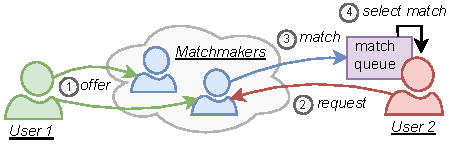
\includegraphics[width=\linewidth]{match/assets/matching_protocol_1}
		\caption{Order creation and dissemination.}
		\label{fig:matching_protocol_1}
	\end{subfigure}\vspace{0.5cm}
	\begin{subfigure}{.45\columnwidth}
		\centering
		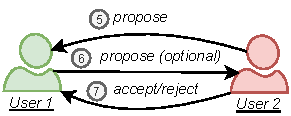
\includegraphics[width=\columnwidth]{match/assets/matching_protocol_2}
		\caption{Order negotiation.}
		\label{fig:matching_protocol_2}
	\end{subfigure}\vspace{0.5cm}
	\begin{subfigure}{.65\columnwidth}
		\centering
		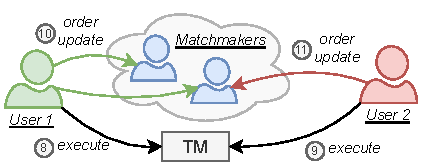
\includegraphics[width=\columnwidth]{match/assets/matching_protocol_3}
		\caption{Match execution and order updates}
		\label{fig:matching_protocol_3}
	\end{subfigure}
	\caption{High-level overview of the MATCH protocol and the message exchange between users and matchmakers.}
	\label{fig:match_data_flow}
\end{figure*}

\section{The MATCH Protocol}
\label{sec:protocol}
We visualize the MATCH protocol and the message exchange between users and matchmakers in Figure~\ref{fig:match_data_flow}.
The key idea behind our protocol is matchmakers only inform users about matches, and that users negotiate a trade directly with counterparties.
%In summary, the protocol proceeds as f.
First, users send new offers and requests to one or more matchmakers (step \circled{1} + \circled{2}).
Matchmakers match incoming orders with existing orders in their order books and notify users about potential matches (step \circled{3}).
Users aggregate potential matches of a specific order in a match queue.
Some period after receiving the first match for a specific order, a user starts to process matches in the associated match queue (step \circled{4}), starting with the best match, and negotiates with the user behind the matched order (step \circled{5} - \circled{7}).
When the negotiating parties reach a trade agreement (in other words, intend to fulfil their orders with each other), they execute the negotiated trade agreement by sending it to the TM (step \circled{8} + \circled{9}).
The negotiating parties then inform the matchmakers about the executed trade so they can update the state of the affected orders accordingly (step \circled{10} + \circled{11}).
The matchmakers are also informed about a negative outcome during the negotiation process.
If an order is still open, a user selects the next best item from the associated match queue, if it is non-empty, and initiates the next negotiation process.
This repeats until the match queue is empty or the order is completed.
The steps in the MATCH protocol are now further explained.

\begin{lstlisting}[language=json,firstnumber=1,float=b,caption=An order in a ride-hailing market (in JSON format).,label=lst:order_example]
{	"timestamp": "2020-02-24T09:09:19+0000",
	"type": "RIDE",
	"timeout": 3600,
	"is_offer": false, // request for transportation
	"public_key": "82ae2f8f0c473cbdf63b920...",
	"signature": "d54af87c8f8e6d917729d14...",
	"identifier": 5,
	"quantity": 1,
	"data": {
		"latitude": "40.712776",
		"longitude": "-74.005974"
	}
}
\end{lstlisting}

\subsection{Order Creation}
\label{sec:order_creation}
In MATCH, users create new orders to indicate their willingness to buy or sell resources, services and assets.
Listing~\ref{lst:order_example} exemplifies the structure of an order in MATCH that specifies a transportation request in a ride-hailing market.
This order, in JSON format, includes the waiting location of the order creator in the \texttt{data} field.
The content of the \texttt{data} field is flexible and depends on the context in which the order is created.
It can contain many attributes and constraints that affect how the order is matched.
Each order has a \texttt{type} field which is a string value indicating the type of the order.
The order type is used by matchmakers to apply the right policies for validation and matching, and to store the order in the appropriate order book.
In Listing~\ref{lst:order_example}, the \texttt{RIDE} type indicates an order in a ride-hailing market.
Similarly, an order with type \texttt{EUR/USD} can indicate an order trading Euro for Dollar.
The \texttt{is\_offer} field is a flag that indicates whether the order is an offer or a request.
%An order contains the following fields: one or more attributes, the order creation timestamp, the order timeout, the public identity of the order creator, a digital signature, the type of the order (offer or request) and a unique identifier.
%To ensure a generic description of offers and requests, each order contains attributes, which are primitive data types such as numbers or text.
%In a ride-hailing market, created orders usually contain at least two numerical attributes that indicate the location of a driver or a passenger (in the form of a longitude and a latitude coordinate).
%This generic description of orders is also adopted by other systems in the domain~\cite{veit2003matchmaking}.
The identifier in an order is an integer value that indicates the position of the order in the sequence of all orders created by that user.
Together with the public key of the order creator, it uniquely identifies an order in the network.
The digital signature in an order allows matchmakers to verify its authenticity.
Inclusion of the \texttt{timeout} value prevents orders from being included in order books for an indefinite amount of time.
Finally, each order has a quantity, which is an integer value that specifies the amount of assets, services or resources being offered or requested.
After creation, a user serializes the order in an \texttt{order} message and sends it to matchmakers.
%With the inclusion of the public identity of the order creator and a digital signature, others can verify the authenticity of new orders and incoming messages from the network.
%We assume that each peer involved in the MATCH protocol owns a digital key pair, used when signing or verifying orders and messages.
%Moreover, we assume that digital signatures cannot be forged and that messages will eventually be delivered, if resubmitted often enough.

%A trader $ t $ creates a new order $ O $ as follows.
%First, $ t $ constructs either an \texttt{offer} or \texttt{request} message containing all fields of the order in serialized form, excluding its digital signature.
%$ t $ then signs the message, appends the signature to it, and sends it to one or more matchmakers.
%How $ O $ is exactly disseminated to matchmakers depends on the implemented order dissemination policy (see Section \ref{subsec:overlay_logic}).
%Upon reception of an incoming \texttt{offer} or \texttt{request} message, a matchmaker first validates the digital signature and the correctness of the order, according to a validation policy (Section \ref{subsec:overlay_logic}).
%If the incoming order is valid, it will be inserted in the order book of the matchmaker and immediately matched.

Users can cancel an open order, say $ O $, at any time by sending a \texttt{cancel} message with the identifier of $ O $ and its public key to matchmakers.
A \texttt{cancel} message for $ O $ should be sent to the same matchmakers as the \texttt{order} message that contained the description of $ O $.
Therefore, users keep track of the matchmakers to which they have sent an \texttt{order} message.
Upon reception of a \texttt{cancel} message, matchmakers remove the cancelled order from their order book.
%The MATCH protocol supports the cancellation of orders.
%When a matchmaker receives a \texttt{cancel} message for $ O $, it should remove $ O $ from its order book.

%\begin{figure}[t]
%	\centering
%	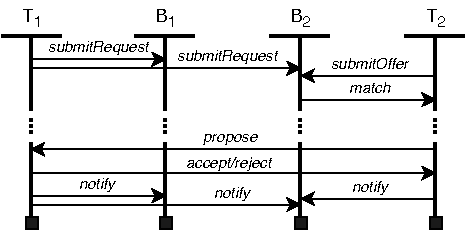
\includegraphics[width=\linewidth]{assets/sequence}
%	\caption{Sequence diagram of the messages exchanged between users and matchmakers in MATCH.}
%	\label{fig:match_sequence}
%\end{figure}

%\begin{figure*}[t]
%	\centering
%	\begin{subfigure}{.33\linewidth}
%		\centering
%		\includegraphics[width=.95\linewidth]{example-image-a}
%		\caption{Accuracy (adaptive $ f $)}
%		\label{fig:taxi_effectiveness_dynamic}
%	\end{subfigure}%
%	\begin{subfigure}{.33\linewidth}
%		\centering
%		\includegraphics[width=.95\linewidth]{example-image-b}
%		\caption{Bandwidth ($ f = 30 $)}
%		\label{fig:taxi_bandwidth_static}
%	\end{subfigure}%
%	\begin{subfigure}{.33\linewidth}
%		\centering
%		\includegraphics[width=.95\linewidth]{example-image-c}
%		\caption{Bandwidth (adaptive $ f $)}
%		\label{fig:taxi_bandwidth_dynamic}
%	\end{subfigure}
%	\caption{The influence of the network size, adversarial rate and message reach on the probability that a broker successfully match a compatible offer and request in MATCH.}
%	\label{fig:dissemination_strategy_experiments}
%\end{figure*}

\begin{figure}[t]
	\centering
	\includegraphics[width=.8\linewidth]{match/assets/matching_idea}
	\caption{The intuition behind order dissemination in MATCH.}
	\label{fig:matching_idea}
\end{figure}

\subsection{Order Dissemination}
\label{sec:order_dissemination}
%We now present the order dissemination model of MATCH.
In the replicated matchmaking model proposed in Section~\ref{sec:towards_fair_reliable_matchmaking}, a new order is disseminated to all matchmakers.
%This is not a scalable approach.
%Our replicated broker model discussed in Section \todo{X} assumes that each peer disseminates a new order to all available brokers.
We now address concern 2 from~Section~\ref{sec:towards_fair_reliable_matchmaking} and show how to considerably decrease the fanout of \texttt{order} messages (i.e., the number of matchmakers that a specific \texttt{order} message reaches) while still ensuring a high probability that a new order reaches a matchmaker with the current best matching order in their order book.
Specifically, we send a new order to a random subset of all matchmakers.
%Figure \ref{fig:matching_idea} illustrates the intuition behind this idea.
Let $ R_{req} $ and $ R_{off} $ indicate the sets of matchmakers that receive a specific request and offer, respectively.
The probability that at least one matchmaker will receive both a specific offer and request quickly goes to one as the order fanout increases, even when the order fanout is low compared to the number of matchmakers.
Figure~\ref{fig:matching_idea} shows the intuition behind this idea.
This phenomena is also known as the \enquote{birthday paradox} and is in practice exploited when computing hash collisions or when detecting a double spend attack in the Bitcoin network~\cite{schreiber2020k}.

Determining to how many matchmakers a new order is sent, is key.
In particular, we are interested in computing the probability that at least one matchmaker receives a matching offer and request.
If we consider a network with 1'000 matchmakers where new orders are disseminated to 50 matchmakers, this probability is given by $ \frac{1000-50}{1000} \cdot \frac{1000-50-1}{1000} \cdots \frac{1000-50-49}{1000} $.
%We indicate the set of matchmakers receiving a particular request and offer, as $ R_{req} $ and $ R_{off} $, respectively.
The probability that there is at least one matchmaker amongst all $ m $ matchmakers receiving both an offer and a request, with order fanout $ f $, is equal to:
%One of the problems of decentralized matchmaking is to ensure a sufficient amount of order duplication, while avoiding a network-wide dissemination of new orders (see Section \ref{subsec:problem_formulation}).
%Our solution is to send new offers and requests to $ f $ unique matchmakers, such that the probability that no matchmaker receives both this offer and request is low.
%We call $ f $ the order fanout.

\begin{equation}
P(R_{req} \cap R_{off} \neq \emptyset) = 1 - \mathlarger{\prod}_{i=0}^{f-1} \big(\frac{m - f - i}{m}\big)
\label{eq:dissemination}
\end{equation}

The value of $ P(R_{req} \cap R_{off} \neq \emptyset) $ quickly increases when $ f $ increases.
Even if $ m = 100'000 $ and $ f = 500 $ (i.e., orders are sent to only 0.5\% of all matchmakers), the probability that at least one matchmaker receives both a matching offer and a request, is already 97.7\%.
In this setting, it reduces the required fanout of an \texttt{order} message from 200'000 (when disseminating a new order to all matchmakers) to merely 1'000, thus significantly reducing the network traffic required for order dissemination.
%Figure \ref{fig:matching_idea} illustrates the intuition behind this idea.
%Applying the idea of Equation~\ref{eq:dissemination} requires an intuition on the total number of matchmakers, which can either be fixed by the software developers or be inferred using network estimation techniques~\cite{shames2012distributed}.
Note that the value of $ m $ is known to users in MATCH since they possess a list of all matchmakers.
We envision that the MATCH software uses a default target value for $ P(R_{req} \cap R_{off} \neq \emptyset) $ (fixed to 0.95 in our experiments).
Depending on the application domain and the number of incoming match messages, users can increase or decrease the fanout as they see fit.
%In practice, the value of $ f $ should be tuned conservatively to account for network failures and matchmakers that are unreachable.
%Our evaluation (Section~\ref{sec:experiments}), we show that this dissemination strategy still results in a near-optimal matching of orders.

%Equation~\ref{eq:dissemination} assumes full network connectivity and an absence of adversarial brokers.
%Since these assumptions are unrealistic, we conduct simulations to better understand the properties of our order dissemination strategy when considering adversarial matchmakers.
%In particular, we experiment with the effects of the network size, fraction of adversarial matchmakers in the network and the reach of orders.
%These results are visualized in Figure~\ref{fig:dissemination_strategy_experiments}.\todo{explain}

\textbf{Malicious Matchmakers.}
Equation~\ref{eq:dissemination} assumes that all matchmakers in the set $ R_{req} \cap R_{off} $ follow the protocol and actually inform order creators when receiving matching orders.
This assumption violates our threat model since malicious matchmakers can respond with sub-optimal matches, or not respond with matches at all.
Therefore, we modify Equation~\ref{eq:dissemination} to account for the situation where a fraction $ r $ of all matchmakers is malicious.
Intuitively, this situation would require a higher value of $ f $ in order to reach at least one honest matchmaker.
%We adjust Equation~\ref{eq:dissemination} .
%We model a malicious matchmaker as a peer that does not respond to incoming offers and requests that match.
%Its behavior is therefore indistinguishable from being offline.
%This also accounts for the situation where a malicious matchmaker matches according to selfish interest, which can be considered as \enquote{invalid} matches.
Given a fraction of malicious matchmakers $ r $, $ P(R_{req} \cap R_{off} \neq \emptyset) $ is now equal to:

\begin{equation}
P(R_{req} \cap R_{off} \neq \emptyset) = 1 - \mathlarger{\prod}_{i=0}^{f-1} \big(\frac{(m - \left \lfloor{(1-r)f}\right \rfloor - i}{m}\big)
\label{eq:malicious_dissemination}
\end{equation}

%Equation~\ref{eq:malicious_dissemination} now accounts for matchmakers that are  who are not informing users about possible matches for their order, either intentionally (e.g., when hiding matches) or unintentionally (e.g., when the matchmaker has crashed).
We show in the next subsection that this is an appropriate modelling of malicious matchmakers.
The rationale behind this model is as follows.
The quality of matches from malicious matchmakers is likely to be lower compared to those received from honest matchmakers.
Therefore, there is a high probability that the effect of malicious matchmakers is negated upon receiving matches from an honest matchmaker, since a user will process the matches of honest matchmakers first.
Reaching honest matchmakers in the presence of malicious matchmakers requires a higher fanout value.

%A matchmaker immediately matches incoming, valid orders with existing ones in their order book.
%Orders are matched according to a matching policy, discussed in Section \ref{subsec:matching_engine}.
%For instance, in a ride-hailing market like Uber, a bid order created by a passenger is matched against only one ask order created by a driver.
When a matchmaker receives an \texttt{order} message describing an order $ O $, it matches $ O $ with existing orders in its order book with the same type, according to a matching policy (see Section~\ref{sec:architecture}).
For each order matched against $ O $, the matchmaker constructs a \texttt{match} message and sends it to the user that created $ O $ (step \circled{3} in Figure~\ref{fig:match_data_flow}).
A \texttt{match} message contains the full specifications of the matched orders, and the network address of the user behind the matched order.
This network address is used by the receiver of the \texttt{match} message to initiate the order negotiation process with the user behind the matched order.
%This message is then digitally signed by $ m $ and sent to the trader that initially created $ O $.\todo{why no reservation?}

%\begin{figure}[t]
%	\centering
%	\includegraphics[width=\linewidth]{assets/matching_idea}
%	\caption{Intuition behind the order dissemination strategy to brokers in MATCH.}
%	\label{fig:matching_idea}
%\end{figure}



%If the order fanout is relatively large (say $ f \geq 100 $), the message dissemination of \texttt{offer}, \texttt{request} and \texttt{CancelOrder} messages differs.
%Instead of sending a new message to $ f $ matchmakers directly, the message is first sent to some matchmakers, who then relay the message to other matchmakers.
%The number of hops that a message traverses is specified by a \emph{TTL} value included in the message.
%Upon receiving a new order from the network, the \emph{TTL} value is decremented by one and only forwarded if \emph{TTL} > 0.
%Our implementation supports gossiping-based message dissemination.

%We now present two basic order dissemination policies, based on the idea in Figure \ref{fig:matching_idea}.

%\textbf{Fixed broadcast (FIXEDBC)} - 
%The fixed broadcast policy, also called \texttt{FIXEDBC}, disseminates a new order to the same $ f $ unique matchmakers every time.
%This set should be fixed when a trader has discovered at least $ f $ matchmakers.
%The matchmakers selected by a trader that creates a large number of new orders have to receive and match incoming orders.
%Additionally, each broadcast order contains a \emph{TTL} value which indicates the maximum number of hops a new order traverses.
%Upon receiving a new order from the network, the \emph{TTL} value is decremented by one and forwarded if \emph{TTL} > 0.
%In this policy, load balancing is not as evenly spread as in the random broadcast policy: matchmakers withing \emph{TTL} hops of a trader that frequently submits orders will incur a higher load.

%The key difference between the random and neighborhood broadcast policies is that the destination set of orders in the latter policy is static.
%Subsequent orders, created by the same trader, should be inserted in the order books of the same matchmakers when neighborhood broadcast is used.


%\textbf{Random broadcast (RANDBC)} - 
%Under the random broadcast policy, also called \texttt{RANDBC}, traders send subsequent orders to $ f $ random, unique matchmakers every time.
%Assuming that these $ f $ matchmakers are uniformly sampled from the network, this policy has better load balancing properties since different matchmakers are selected each time traders broadcast a new order.
%This policy requires traders to discover more matchmakers when bootstrapping in the network, compared to the \texttt{FIXEDBC} policy.
%A potential trade off of this policy is matching effectiveness, since orders might not be matched in an optimal manner, depending on the matchmakers a specific order is sent to.
%We will discuss how to effectively pick the value of $ n $ further in this section.

\subsection{Match Queue}
\label{sec:match_queue}
Upon receiving a \texttt{match} message from a matchmaker, a user contacts the creator of the matched order and initiates a negotiation process (further discussed in Section~\ref{sec:order_negotiation}).
%After creating a new order, a trader can receive multiple \texttt{match} messages within a short period of time.
A potential strategy is that the user immediately contacts another user upon the arrival of a \texttt{match} message.
This possibly minimizes the time for an order to be completed.
However, this strategy leaves the user vulnerable to an attack where a malicious matchmaker is the first to send a specific \texttt{match} message to a user, which immediately triggers the negotiation process.
The quality of the received match described by the \texttt{match} message might be poor and the user might have received a match with a higher quality if it would have waited for additional matches from honest matchmakers.

\begin{figure*}[t]
	\centering
	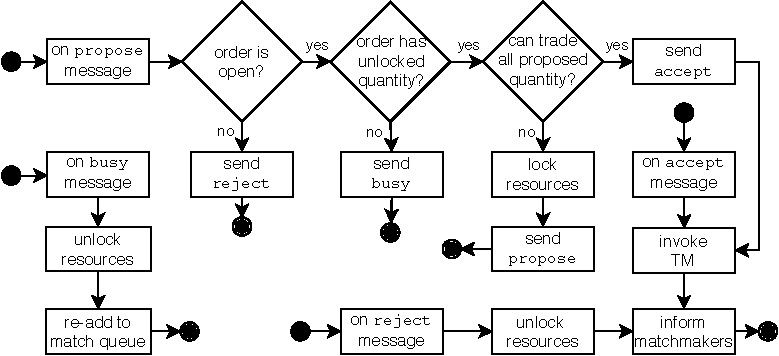
\includegraphics[width=\linewidth]{match/assets/negotiation_diagram}
	\caption{The flow diagram (in UML format) when receiving a message during the negotiation process for a specific order.}
	\label{fig:order_negotiation_diagram}
\end{figure*}

To address this issue, incoming \texttt{match} messages for a specific order are first stored in a \emph{match queue}.
When a user receives the first \texttt{match} message for one of its offers (or requests), say $ O $, it creates a new match queue for $ O $.
Each entry in the match queue of offer (or request) $ O $ is a tuple $ (a, R) $ where $ R $ is a request (or offer) that matches with offer (or request) $ O $.
$ a $ indicates the number of failed negotiation attempts for $ R $.
The value of $ a $ is locally tracked by each user.
%The number of retries indicates how many times we unsuccessfully negotiated with the creator of $ O_2 $.
Removing items from the match queue is first based on $ a $ (item with a lower value of $ a $ have higher priority) and is then based on the quality of the match (the user prioritizes negotiation of matches with higher quality).
The quality of a match is an application-specific metric that can be considered as the \enquote{distance} between an offer and a request, and is computed by the matching policy.
An incoming \texttt{match} message can be inserted in multiple match queues, e.g., in the match queues for offers or requests with the same type and similar specifications.
%$ r $ is initially zero and is incremented by one each time trade negotiation fails (see Section~\ref{sec:order_negotiation}).
%Specifically, when a trader receives a \texttt{RejectTrade} message with this reason from the creator of $ O_2 $ during trade negotiation for his own order $ O_1 $, it adds the entry $ (r + 1, O_2) $ to the priority queue of $ O_1 $.
%Since a trading partner might have quantity reserved in their order that is released later, we try to send another trade proposal later in this situation.

%User store incoming \texttt{match} messages for a duration $ W_match $, after having received the first \texttt{match} message for a specific order.
Before a user starts to select items from a match queue, it waits for some duration $ W_{match} $, which we call the \emph{match window}.
The value of $ W_{match} $ should be carefully considered: a higher value of $ W_{match} $ increases the probability of receiving more and better matches but adds to the order completion time since a user has to wait longer before starting order negotiations.
Decreasing $ W_{match} $, however, might result in missing better matches.
$ W_{match} $ also depends on the link latency of the peer-to-peer network.
Furthermore, $ W_{match} $ is influenced by the trading domain, e.g., passengers in a ride-hailing market can usually tolerate an additional wait time of a few seconds, whereas this increase might be unacceptable when a user quickly wants to buy some assets in response to price fluctuations in an asset market.
When the match window expires, a user removes the entry $ (a, R) $ with the best quality from the match queue and initiates the order negotiation process with the user that created $ R $.
%Users prioritize the selection of items from the match queue first by the quality of the match, and then by $ r $.
%To prevent traders from sending out \texttt{ProposeTrade} messages at roughly the same time (and thus increasing load on individual traders), we introduce a small \emph{propose window} $ W_p $ which is a random duration between the removal of an entry from a match queue, and sending out a \texttt{ProposeTrade} message.
%Only when negotiation for an order fails or succeeds, the next entry is removed from the appropriate match queue, until the order is either canceled, expired or completed.
%If order $ O $ is completed, the match queue associated with $ O $ is deleted.

\subsection{Order Negotiation}
\label{sec:order_negotiation}

In MATCH, users negotiate about their orders with other users.
This negotiation approach increases resilience against malicious matchmakers since rational users choose to negotiate about the best incoming matches in order to get the best deal.
When two negotiating users reach a trade agreement, both users send the agreement to the TM, upon which the trade is executed.
This approach addresses question 1 in Section~\ref{sec:towards_fair_reliable_matchmaking} and avoids the need for network-wide consensus.

We now elaborate on the negotiation procedure between two users.
In the following, we assume that user $ U_1 $ created offer $ O $, user $ U_2 $ created request $ R $, and these two orders match.
Now, $ U_2 $ has received a \texttt{match} message from a matchmaker, informing $ U_2 $ about matching offer $ O $.
This puts entry $ (a, O) $ in the match queue associated with $ R $.
Order negotiation, based on match queue entry $ (a, O) $, starts by $ U_2 $ locking quantity in request $ R $.
How much quantity is locked depends on the available quantities in both $ O $ and $ R $.
Specifically, $ U_2 $ proposes to trade as much available quantity as possible, given the specifications of $ O $ and $ R $.
Explicitly locking quantity in an order prevents a user from engaging in parallel negotiations for the same resources.
MATCH does not enforce the locking of quantity since we assume that rational users will correctly manage their orders.
After locking the quantities in $ R $, $ U_2 $ sends a \texttt{propose} message to $ U_1 $, containing the full specifications of $ R $, the identifier of $ O $, and the proposed quantity to trade.

Figure~\ref{fig:order_negotiation_diagram} shows the control flow in UML format when a user receives specific messages during the order negotiation process.
We elaborate the negotiation process between users $ U_1 $ and $ U_2 $ according to Figure~\ref{fig:order_negotiation_diagram}.
When $ U_1 $ receives a \texttt{propose} message from $ U_2 $, it first checks if its offer $ O $, which identifier is contained in the \texttt{propose} message, is still open.
If $ O $ is expired, has been cancelled, or has been completed already, $ U_2 $ immediately responds with a \texttt{reject} message, containing the reject reason.
When $ U_2 $ receives the \texttt{reject} message from $ U_1 $, it unlocks the locked quantity for that negotiation and selects the next entry from the match queue of its request $ R $.
Since matchmakers might have outdated information about $ O $ (e.g., when $ O $ has been completed but the matchmaker has not been notified about this event), $ U_2 $ forwards the \texttt{reject} message to the matchmakers that informed $ U_2 $ about the match with $ O $.
Matchmakers then update the state of $ O $ accordingly when receiving a \texttt{reject} message.

If offer $ O $ is open, $ U_1 $ first determines if the incoming proposal is acceptable.
This step depends on the trading domain and specifically on the application-specific data in the order.
For example, a matchmaker in a ride-hailing market can establish a valid match between a passenger and driver.
However, this match might be unacceptable for one of the matched parties (e.g., when the geographic separation between the parties is too large).
If $ U_1 $ finds the proposal unacceptable, it sends a \texttt{reject} message to $ U_2 $.

If the proposal is acceptable, $ U_1 $ checks if it has any unlocked quantity in the offer $ O $.
If there is no unlocked quantity available for trade, $ U_1 $ responds with a \texttt{busy} message to $ U_2 $, indicating that it currently has no room for negotiation.
In this situation, $ U_1 $ is already engaged in negotiations for that order with other users.
Upon receiving a \texttt{busy} message, $ U_2 $ unlocks the locked quantity in $ R $ and re-adds the entry associated with the failed negotiation to the match queue of $ R $, incrementing $ a $ by one.
Re-adding this entry to the match queue will cause $ U_2 $ to initiate a negotiation with $ U_1 $ again later.
To prevent a user from immediately retrying a failed negotiation, a user waits a random period (between 1 and 2 seconds) before sending out another \texttt{propose} message when processing a match queue entry with $ a > 0 $.

If offer $ O $ has unlocked quantity, $ U_1 $ checks whether the full proposed quantity can be traded.
If so, $ U_1 $ sends an \texttt{accept} message to $ U_2 $, thereby accepting the proposal of $ U_2 $.
$ U_1 $ also forwards the \texttt{accept} message to the matchmakers that proposed the match so they can update the state of this order in their order book.
If the proposed quantity is unavailable in $ O $, $ U_1 $ makes a counter-proposal by locking as much quantity as possible in $ O $ and by sending a \texttt{proposal} message back to $ U_2 $ with this (lower) quantity.
$ U_1 $ and $ U_2 $ keep sending \texttt{propose} messages with differing quantities until one of them responds with either an \texttt{accept} or a \texttt{reject} message.

%During the second phase of the matching protocol traders negotiate a trade based on an incoming \texttt{match} message (see Figure \ref{fig:matching_protocol_2}).

%This phase starts when a trader, say $ t_1 $, receives a \texttt{match} message for its order $ O_1 $ from a matchmaker $ m $ that matched $ O_1 $ with another order $ O_2 $, created by $ t_2 $.
%When a trader receives a \texttt{match} message, it contact the trader behind the matched order directly, and try to negotiate a trade.
%This process is visualized in Figure \ref{fig:matching_protocol_2} and always involves the trader behind a matched ask and bid order.
%The recipient $ t_1 $ of a \texttt{match} message that matches order $ O_1 $ (created by $ t $) with another order $ O_2 $ (created by $ t_2 $) first checks whether his order is still open (since it could have been fulfilled already by other orders).
%If $ O_1 $ is expired, completed, or canceled, $ t_1 $ immediately sends a \texttt{DeclineMatch} message back to $ m $ and $ m $ then removes $ O_1 $ from its order book.
%Otherwise, $ t_1 $ reserves a part of (the assets, resources or services in) $ O_1 $ and sends a \texttt{ProposeTrade} message to $ t_2 $.
%This message contains full specifications of $ O_1 $ and a trade proposal with a quantity $ q $.
%During this phase, the sender digitally signs all their outgoing messages.

%When $ t_2 $ receives a \texttt{ProposeTrade} message from $ t_1 $, it first checks the status of its order $ O_2 $.
%If this order is expired, completed or canceled, $ t_2 $ immediately sends a \texttt{RejectTrade} message back to $ t_1 $.
%The same happens when there is no unreserved quantity available in $ O_2 $, e.g., when $ t_2 $ has an outstanding trade proposal with another trader.
%A \texttt{RejectTrade} message contains the reason why the trade proposal is rejected.
%If $ O_2 $ has at least $ q $ available quantity, $ t_2 $ sends an \texttt{AcceptTrade} message to $ t_1 $.
%Otherwise, if $ O_2 $ has available quantity but less than $ q $, $ t_2 $ can send a \texttt{CounterTrade} message to $ t_1 $, proposing an alternative quantity to trade.
%$ t_1 $ either accepts or rejects a counter proposal by responding with a \texttt{AcceptTrade} or \texttt{RejectTrade} message, respectively.
%At most, three messages are exchanged between $ t_1 $ and $ t_2 $ during this phase.
%At this point, $ t_1 $ and $ t_2 $ have either negotiated a trade, or one of the parties declined a trade proposal.

It could be that one of the involved parties does not respond during a negotiation, e.g., to deliberately lock quantity in the orders of another user.
%In this case, $ t_1 $ will never receive a response from $ t_2 $.
To address this situation, all outgoing messages during order negotiation have a fixed \emph{negotiation window}, indicated by $ W_{neg} $, after which the user leaves the negotiation.
When this window expires, any locked quantity for this negotiation is released and incoming messages regarding the expired negotiation are ignored.

%We prevent this by having a trader aggregate multiple incoming \texttt{matches} for the same order before sending out trade proposals.
%After receiving the first \texttt{match} message for a specific order, a trader waits for a fixed duration in seconds which we refer to as the \emph{matching window}, denoted by $ w $.
%A high value of $ w $ increases the probability of receiving good matches but delays the order completion process since one has to wait longer before sending out trade proposals.
%On the other hand, a small $ w $ might lead to missing better matches.

%\subsection{Avoiding Full Replication}
%TODO

%\section{The MATCH Protocol}
%\label{sec:protocol}
%To ensure correct order management (problem I), we design a three-phase protocol, named MATCH.
%We first briefly introduce the MATCH protocol and its phases, and then provide a more detailed description per phase.
%The design of the MATCH protocol is inspired by prior work of Raman et al., which proposes a related protocol to match resources and jobs in a centralized matchmaking environment~\cite{raman1998matchmaking}.

%In phase I, order creators submit new offers and requests to matchmakers and matchmakers notify these creators about potential trading parties with \emph{match notifications}.
%When receiving a match notification from a matchmaker, an order creator starts to negotiate directly with the matched party (phase II) and informs matchmakers about the outcome of the trade negotiation (phase III).
%Since order creators will collect incoming match proposals and process them accordingly, this protocol ensures correct behavior in the situation where multiple matchmakers match the same order.
%To prevent orders from being settled multiple times, matchmakers inform traders about potential trading partners, upon which traders start to negotiate a trade with the matched counterparty.\todo{why matchmaking at all?, pre-aggregate of information, exhaustive search}
%Since the creator behind an order will determine to which matches it responds and ensures their order is not fulfilled multiple times, different matchmakers can propose the same match to this order creator simultaneously. % it addresses the problem where the same order is matched by multiple matchmakers.

%We embed this  embedded in the design of the MATCH protocol, visualized in Figure \ref{fig:matching_protocol}.
%First, traders send new orders to matchmakers and  matchmakers match the orders of two traders.
%Next, a trader that is informed about a potential match directly contacts the matched counterparty and proposes to trade.
%When the trade is finished, the involved parties notify the matchmaker and their order books are then updated accordingly.

\subsection{Match Execution and Order Updates}
Upon reaching a trade agreement between two negotiating users, it should be executed by the trading mechanism.
To execute a trade agreement, one party sends the \texttt{propose} message to the TM and the other party sends the \texttt{accept} message to the TM (step \circled{8} and \circled{9} in Figure~\ref{fig:match_data_flow}).
Each message contains the digital signature of its creator.
The TM executes the trade after having received both these messages.
%Both users then internally update their order.
Next, each involved party individually inform the matchmakers that originally received their order about the match execution by sending an \texttt{update} message (step \circled{10} and \circled{11} in Figure~\ref{fig:match_data_flow}).
This message contains the order with an updated quantity, specifying the new interests of the order creator after the match has been executed.
The \texttt{update} message contains an order with quantity 0 if it has been completed.
%When $ t_1 $ and $ t_2 $ agree to trade, the trade should be executed by actually exchanging assets, services or resources.
%We assume that a negotiated trade is executed by an application-specific trading mechanism (its specifications are discussed in Section \ref{subsec:trading_mechanism}).
%When a trade has successfully been executed between $ t_1 $ and $ t_2 $, both parties notify the original recipients of the \texttt{offer} or \texttt{request} messages that contained $ O_1 $ or $ O_2 $, by broadcasting a signed \texttt{TradeComplete} message.
%A \texttt{TradeComplete} message contains full specifications of both orders, and the details of the executed trade between $ t_1 $ and $ t_2 $.
%Both $ t_1 $ and $ t_2 $ broadcast a \texttt{TradeComplete} message to the matchmakers where they initially sent their \texttt{ask} or \texttt{bid} message to.
Upon receiving an \texttt{update} message, matchmakers update the state of the changed order accordingly and remove orders that have been completed.

%If trade negotiation has failed or a trade proposal did time out, one of the involved parties (either $ t_1 $ or $ t_2 $) notifies the matchmaker $ m $ about the outcome by sending a \texttt{DeclineMatch} message, containing the reason of the failed trade negotiation.
%If a \texttt{DeclineMatch} message indicates that either $ O_1 $ or $ O_2 $ is completed, canceled, or expired, $ m $ removes this order from their order book.
%A \texttt{DeclineMatch} message is also sent back to $ m $ if the actual trade fails for reasons specific to the trading mechanism (see Section \ref{subsec:trading_mechanism}).

%\subsection{Order Book Synchronization}
%In MATCH, matchmakers periodically synchronize orders in the order book with other matchmakers.
%We refer to the duration between subsequent synchronizations of a single matchmaker as the \emph{synchronization window} $ W_{sync} $.
%A matchmaker $ m_1 $ synchronizes their order book with matchmaker $ m_2 $ as follows: periodically, $ m_1 $ sends a \texttt{sync} message to a random other matchmaker, say $ m_2 $.
%This message contains a Bloom filter $ B $, initialized with the identifiers of all offers and requests in the order book of $ m_1 $.
%The false positive rate of $ B $ is fixed to 5\%.
%When $ m_2 $ receives a \texttt{sync} message, it iterates over all offers and requests in its order book and assembles a set with order identifiers that have no membership in $ B $.
%To avoid synchronization of the entire order book, $ m_1 $ samples a random subset with $ b $ orders, where $ b $ is called the synchronization batch size.
%Upon reception of $ B $, $ m_2 $ sends up to $ b $ individual \texttt{order} messages to $ m_1 $.

%Which orders are being synchronized depends on an \emph{synchronization policy}.\todo{to BF or not to BF?}

%A matchmaker that wants to synchronize their order book with another peer first sends a message that contains two bloomfilters: one filled with the IDs of active orders in the order book, and another one that is filled with the IDs of canceled orders.\todo{why cancelled orders?}
%The receiving party now sends missing orders to the initiating party.

%\textbf{No synchronization} -
%While (periodic) order synchronization potentially increases matching effectiveness, the additional communication outweighs the increased matching effectiveness in specific situations.
%For example, order synchronization is less effective when a new order is already disseminated to a significant fraction of all matchmakers.
%Therefore, we also consider a policy where orders are not synchronized at all.
%No synchronization reduces communication costs but potentially leads to the miss of better matches.

\subsection{Privacy Considerations}
We end our protocol description with a few notes on privacy.
In MATCH, full order details are shared with and amongst matchmakers.
While this is standard for application domains such as blockchain marketplaces, it is undesirable for some application domains such as financial markets.
We note that the \texttt{data} field of an order in MATCH can be fully specified by the system designers.
Therefore, the content of orders, and the quantity field, can be subjected to cryptographic protocols such as encryption.
Only when an agreement has been reached between two parties, the order specifications can be revealed between the two interacting parties.
To leverage the functionality of the match queue, however, it is desirable that incoming orders can be totally ordered.

There are some privacy-preserving solutions for matchmaking in particular application domains, such as ride-hailing.
ORide, for example, leverages homomorphic encryption to build a full protocol for privacy-preserving ride sharing~\cite{pham2017oride}.
We believe that, whether or not with additional research, the underlying ideas of existing solutions such as ORide can increase the privacy aspects of decentralized matchmaking.

\section{The MATCH Middleware Architecture}
\label{sec:architecture}
We now present the MATCH middleware architecture, visualized in Figure~\ref{fig:matching_architecture}.
Each user and matchmaker deploy a single instance of the MATCH middleware as a shared runtime library.
Communication with the middleware by external applications proceeds through an API, which specifications are included in our open-source implementation.
We now elaborate on the components in the MATCH middleware architecture.
%We now present the architecture of MATCH, our distributed order matching mechanism.
%The overall architecture and information flow is presented in Figure \ref{fig:matching_architecture}.
%We briefly elaborate on the individual components.

\textbf{Network layer.}
The network layer passes incoming messages to the MATCH overlay logic and routes outgoing messages to their intended destination.
This layer can be implemented using any networking library with support for peer-to-peer communication and authenticated messaging.
%We should note however that further optimizations can be made in network topology, depending on the domain to which MATCH is applied.
%This lowers generality and re-usability.
%The network has a random topology and each peer $ p $ maintains a connection to $ i $ other random peers.

\begin{figure}[t]
	\centering
	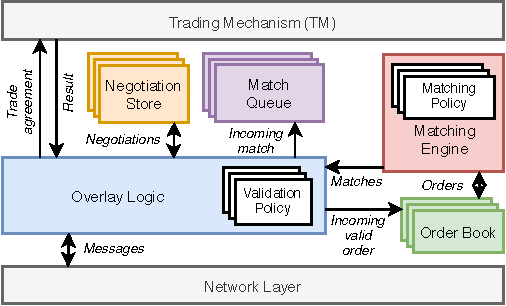
\includegraphics[width=.9\linewidth]{match/assets/matching_architecture}
	\caption{The MATCH middleware architecture.}
	\label{fig:matching_architecture}
\end{figure}

\textbf{Overlay logic.}
The overlay logic processes incoming messages received by the network layer. %, such as new orders, matches and received from the network. % various routines that execute when a specific message is received.
It inserts incoming \texttt{match} messages in the appropriate match queue, discussed in Section~\ref{sec:match_queue}.
It contains policies for order \emph{validation} which specify how the validity of an incoming order with a given type is determined.
The validation policy takes into consideration the attributes in the \texttt{data} field of the order (see Listing~\ref{lst:order_example}), and checks whether they are valid with respect to a trading domain.
For example, a validation policy for orders in a ride-hailing market should check whether the latitude and longitude coordinates are included and within a valid range (-90 to 90).
We envision that developers share the implementation of these policies through some distribution medium (e.g., a website).
To increase the trustworthiness and security of these policies, the policy implementations should be auditable and attestable by other developers and auditors.
These validation policies can then downloaded by users and matchmakers that are interesting in participation within a specific trading domain.
We provide developers the means to create custom validation policies, enabling order validation in different trading contexts.
Incoming orders deemed invalid by the validation policy are discarded and not processed.

%New incoming orders received by overlay logic are first checked for validity; if valid they are dispatched to both the order book (so they can be inserted) and the matching engine, which attempts to find matches for this new order.

\textbf{Order books.}
Each matchmaker can host multiple order books, coloured green in Figure~\ref{fig:matching_architecture}, which store orders with differing types.
For example, MATCH can maintain an asset trading order book that stores orders to buy or sell Euros for Dollars, and another ride-hailing order book that stores transportation requests and ride offers.
Maintaining multiple order books is a key property of MATCH and results in a single and reusable matchmaking solution that can be deployed across different domains.
%New order books are created on demand, based on the type of incoming orders.

\textbf{Matching engine.}
Valid incoming orders are passed to the matching engine, coloured red in Figure~\ref{fig:matching_architecture}.
The matching engine attempts to match incoming offers and requests with existing requests and offers, respectively.
It contains \emph{matching policies} which predicate whether a specific offer and request match, based on the order type and specifications.
%It takes a buy and a sell order as input and determines whether there is a match, based on one or more attributes of these orders.
For example, matchmaking in a ride-hailing market is often based on the geographic distance between a driver and a passenger.
Likewise, asset orders would match if the price of an offer is equal to or lower than the price of a request.
Similar to validation policies, matching policies are published on a website or on another public medium, and can be downloaded by interested matchmakers.
%Matchmaking can also be based on multiple, weighted attributes.
%A match found by the matching engine is passed to the overlay logic, converted into a \texttt{match} message, and send to the order creator.

\textbf{Negotiation stores.}
To correctly process incoming messages from negotiation counterparties, MATCH requires state storage of outgoing messages during order negotiation.
This state is stored in a \emph{negotiation store}, coloured yellow in Figure~\ref{fig:matching_architecture}.
For each negotiation, a new negotiation store is created, a unique identifier is generated, and this identifier is appended to each message associated with this negotiation.
Counterparties are required to include the same identifier in response messages.
Incoming negotiation messages containing an unknown identifier are discarded by users.
Negotiation stores time out after the negotiation window expires, on which the store and its contents are deleted.
%On timeout, the negotiation store is deleted and the overlay logic is notified about this event.

\textbf{Trading mechanism.}
Negotiated trade agreements are passed to the trading mechanism that executes the trade.
We consider this component external to MATCH.
%The trading mechanism requires the implementation of the \texttt{startTrade($ O_1, O_2, q $)} function which expects the two matched orders $ O_1 $ and $ O_2 $, and the agreed quantity to trade ($ q $) as arguments.
The trading mechanism notifies the overlay logic when the trade is executed.
This notification includes one or more transaction identifiers and a boolean value indicating whether the trade was successful or not.
We assume that the trading mechanism provides atomic guarantees: either the full negotiated match is executed or nothing is being executed.
This guarantee is, for example, provided by smart contracts, applications that runs on top of a blockchain (also see Section~\ref{sec:experiments_ethereum})~\cite{luu2016making}.
%The trading mechanism the notifies the overlay logic with the outcome of the trade.
%We consider three different trade outcomes: succeeded, when all assets have successfully been exchange between two parties, or failed, when an error occurred during the trading process.
%The trade outcome is then broadcast to matchmakers (see phase III in Section~\ref{subsec:protocol_phase_3}).

%\section{Model and Formalisms}
%MATCH is middleware that interacts with a peer-to-peer network and market trading mechanism.
%Prior to presenting the architecture of MATCH and the matching protocol, we discuss the model of our peer-to-peer network and trading mechanism.
%We start by defining the specifications and assumptions of the network layer and trading mechanism.
%Next, we formally define the data structures that MATCH requires, including orders, the order book and the matching function.
%These definitions will guide the design of our matchmaking protocol.

%\subsection{Trading Mechanism Model}
%We assume that there is a trading mechanism that handles the execution of a trade between two participants.
%The trading mechanism handles the trading process after two orders have been matched, and ensures that resources, services or assets between the entities that created the matched orders, are traded.
%This process might be executed by one or more centralized entities, e.g. financial institutions that transfers funds from one party to another.
%We assume that the asset exchange mechanism used in the market mechanism is secured against fraud.
%This could for instance be achieved by using atomic swaps where assets are exchanged between blockchain ledgers in a secure and atomic manner. %or a trusted central settlement institution.


%\subsection{Data Structures}
%The goal of MATCH is to match incoming orders in a decentralized manner.
%To keep our mechanism applicable in many market contexts, we specifically do not make assumptions about the content of individual orders.
%We now formally define various data structures which MATCH uses.
%MATCH is built to act as middleware between a peer-to-peer network and a trading mechanism.
%More specifically, we assume a trading environment where assets are being traded.

%First, we provide the definition of an asset.
%An asset represents either a tangible or intangible object with some value, e.g. some dollars, stocks or a taxi ride.
%We formally define an asset as follows:

%\begin{mydef}
%	(Asset) An asset $ A $ is defined as a pair $ (ID, A) $ where $ ID $ is a unique serializable identifier that represents the type of the asset and $ A = (a_1, a_2, ... a_n) $ denotes a set of $ n $ attributes.
%\end{mydef}

%In the context of stock trading, we can define a specific quantity of assets as $ (AAPL, \{amount=23\}) $ to indicate 23 stocks with the $ AAPL $ symbol.
%While an asset might intuitively be thought of as some physical or digital good, we can use Definition X to also model resources or services as assets.
%For example, a service request for transportation to a remote location in a ride-hailing market can be modelled as $ (RIDEREQ, \{pickup=(1, 2), dropoff=(1,2)\}) $.
%The methodology of modelling tangible and intangible assets or resources as digital tokens is a commonly adopted concept within various blockchain-based marketplaces. % approach is very  the "tokenization" of both tangible (physical) and intangible assets.

%In most electronic markets, two types of assets are being exchanged between traders, e.g. two types of currencies.
%Before we define what comprises an order in MATCH, we must first define an asset pair.

%\begin{mydef}
%	(Asset pair) An asset pair $ P = (A_1, A_2) $ is an ordered pair of two assets $ A_1 $ and $ A_2 $ where $ A_1.id $ is lexicographically smaller than $ A_2.id $.
%\end{mydef}

%We can now model the specifications of an asset exchange between two trades as an asset pair.
%For example, if a trader wants to sell 23 stocks of the AAPL symbol for a price of \$40 each, we can model this with the asset pair $ ((AAPL, \{amount=23\}), (EUR, 920)) $.
%With the definition of an asset pair, we can now formalize an order.

%\begin{mydef}
%	(Order)
%	An order $ O_t $ created by trader $ t $ is defined as a tuple $ (P, t_{pk}, i) $ where $ P $ is an asset pair, $ t_{pk} $ the public key of trader $ t $, $ i $ indicates the timeout of the order in milliseconds.
%\end{mydef}

%We now make the distinction between ask (sell) orders and bid (buy) orders.

%\begin{mydef}
%	(Ask order) An ask order $ A_t $ created by trader $ t $ is a sell order $ O_t $ where $ t $ intends to exchange $ O_t.P.A_1 $ for $ O_t.P.A_2 $.
%\end{mydef}

%\begin{mydef}
%	(Bid order) A bid order $ A_t $ created by trader $ t $ is a buy order $ O_t $ where $ t $ intends to exchange $ O_t.P.A_2 $ for $ O_t.P.A_1 $.
%\end{mydef}

%Recall that we restricted an asset pair to be ordered in Definition X.
%This is explicitly done to avoid symmetric orders.
%To elaborate, an ask with asset pair $ (A_1, A_2) $ is equivalent a bid with asset pair $ (A_2, A_1) $.
%To avoid duplication in the market, we enforce an order within the asset pair.

%Matchmakers organize known ask and bids within an \emph{order book}, which we formally define in the following definition.

%\begin{mydef}
%	(Orderbook) An order book $ B_{t1, t2} $ is defined as a set $ \{ O_1, O_2, ... O_n \} $ of $ n $ orders. We denote the size of order book $ B $ as $ |B| $.
%\end{mydef}

%Note that each order has a timeout.
%This attribute is included to prevent orders from being open for an indefinite amount of time and potentially polluting order books across the network.
%In addition, each order is digitally signed by its creator.
%This prevents other traders from creating orders under a different identity.

%Figure \ref{fig:order_book} shows an example of an order book used in a stock trading market, with three bid orders and three ask orders.
%When presenting an order book to traders, ask and bid orders are usually sorted, i.e. based on their price.
%For orders with a price, ask orders are sorted ascending on price and bid orders descending on price in the order book (the best orders are presented first).

%When a trader receives a new ask or bid from the network, it attempts to match this new order with existing orders in the order book.
%We now define a generic matching function, that takes a new order and order book as input, and output a set of orders that match.

%\begin{mydef}
%	(Matching function) A matching function $ M: (O, B) \rightarrow  $ returns matching ask or bid orders in an order book $ B $ for a new incoming bid or ask order respectively.
%\end{mydef}

%At this point, we should remark that the matching function highly depends on the type of assets being traded.
%The matching function usually takes in consideration one or more attributes of the assets defined in the order, e.g. a price in the context of stock trading or a pickup location when matching passengers and drivers a ride-hailing market.
%To illustrate this, assume that a new bid order arrives with a price of \$149.58 and with an amount of 800, and is matched against the content of the order book presented in Figure \ref{fig:order_book}. %, when a new bid order is submitted to the order book in Figure \ref{fig:order_book} , it will be matched with the following ask orders.
%Now, this bid order will be fully matched against the ask orders with ID \#7829 and ID \#7828 and the ask order with ID \#7820 will be partially matched for an amount of 104.
%When two or more orders are matched, their order book entries are updated or they are removed from the order book if the order is fulfilled.

%\section{Implementation Details}
%\label{sec:implementation}
%Request stores are organized in a dictionary with the request identifiers as keys and the individual request stores as values.
%The matching priority queue is implemented as a linked list that remains sorted whenever new entries are added to it.
%Different order books are organized in a dictionary whose keys are the order types, and the values are the individual order books.
%We provide both an implementation of a basic order book and a limit order book, optimized to store orders with pricing information.
%The basic order book structure contains two distinct sets with offers and requests, and can be used to store and match orders with any type of attributes.


%It matches orders first based on price, and then on time since order creation, while prioritizing orders that have been open for a longer time.
%Programmers can add custom matching policies by subclassing the \texttt{MatchPolicy} class and providing an implementation of the \texttt{match(order, order\_book)} method, which takes the order and a order book as parameters, and returns a set of matching orders.
%We provide a basic order validation policy that checks whether an incoming order has not expired yet and is not canceled already.
%Programmers can define advanced validation policies by subclassing the \texttt{ValidationPolicy} class and implementing the \texttt{isValid(order)} method, which takes the order to be validated as parameter and returns a boolean value.

%When a trader broadcasts a new order in the network, they can potentially receive a significant number of \texttt{match} messages within a short period of time, in particular when the order matches with multiple other ones, and the order fanout is large.
%To prevent a high load on a trader, we wait for a random duration between 0 and 1 second before sending an outgoing trade proposal to another trader the first time.
%Subsequent trade proposals to the same trader are queued for a duration between 1 and 2 seconds.
%Depending on the connectivity of the underlying peer-to-peer network, the wait duration might be increased.

%We now present various policies that specify how new orders are sent to matchmakers, and how existing orders are synchronized amongst them.
%In this section, we distinguish between \emph{synchronization} and \emph{dissemination} policies, and discuss each policy type in a separate section.

% Policies:
% - smart broadcast of new order
% - send new order to random matchmakers

% - neighbour sync
% - active sync amongst matchmakers + rand. walk
%

\begin{table}[t!]
	%\footnotesize
	\centering
	\begin{tabular}{|c|c|}
		\hline
		\textbf{Notation} & \textbf{Variable Description} \\ \hline
		$ W_{match} $ & Match window (fixed to 2 seconds) \\ \hline
		$ W_{neg} $ & Negotiation window (fixed to 5 seconds) \\ \hline
		$ m $ & Number of matchmakers \\ \hline
		$ f $ & Order fanout \\ \hline
		$ r $ & Fraction of malicious matchmakers \\ \hline
	\end{tabular}
	\caption{An overview of the variables used in Section~\ref{sec:match_experiments}.}
	\label{table:experiment_parameters}
\end{table}

\section{Experimental Evaluation}
\label{sec:match_experiments}
We implement the MATCH protocol and middleware in the Python 3 programming language, spanning a total of 6.511 lines of source code (SLOC), without comments.
The implementation uses the \texttt{asyncio} library for asynchronous event processing.
The network layer is implemented using our networking library, optimized for building peer-to-peer overlay networks and with built-in support for Network Address Translation (NAT) puncturing and authenticated messaging.\footnote{See \url{https://github.com/tribler/py-ipv8}}
For efficiency, message exchange between users and matchmakers uses UDP.
Order negotiation proceeds using TCP since this flow requires bilateral and reliable message exchange.
All software artifacts of MATCH (source code, tests, and documentation) are available online.\footnote{See \url{https://github.com/Tribler/anydex-core/tree/match-middleware20}}

In Section~\ref{sec:taxi_experiments} and~\ref{sec:asset_trading_experiments}, we subject the MATCH middleware to two workloads for ride-hailing and asset trading, reconstructed from real-world traces.
These experiments demonstrates that MATCH maintains high matching quality, is resilient against malicious matchmakers, and is reusable across different trading domains.
In Section~\ref{sec:experiments_ethereum}, we compare our solution to matchmaking on an Ethereum blockchain and show that MATCH uses considerably less bandwidth and has superior order fulfil latencies.
%Afterwards, we provide a summary with recommendations for each policy and their performance with regard to various system properties.

\begin{figure*}[t]
	\centering
	\begin{subfigure}{.5\columnwidth}
		\centering
		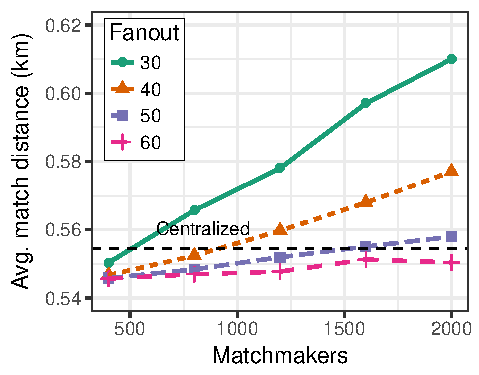
\includegraphics[width=\linewidth]{match/assets/plots/taxi_quality.pdf}
		\caption{Matching quality w. different fanouts $ f $}
		\label{fig:taxi_quality}
	\end{subfigure}%
	\begin{subfigure}{.5\columnwidth}
		\centering
		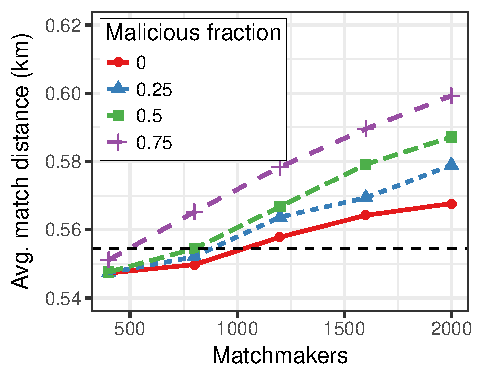
\includegraphics[width=\columnwidth]{match/assets/plots/taxi_fairness_fixed.pdf}
		\caption{Impact of selfish matching ($ f = 50 $)}
		\label{fig:taxi_fairness_fixed}
	\end{subfigure}\vspace{0.3cm}
	\begin{subfigure}{.5\columnwidth}
		\centering
		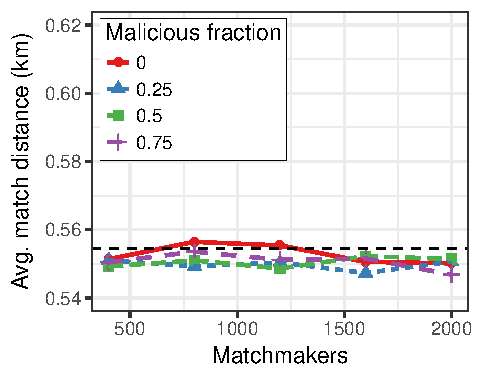
\includegraphics[width=\columnwidth]{match/assets/plots/taxi_fairness_adaptive.pdf}
		\caption{Impact of selfish matching (adaptive $ f $)}
		\label{fig:taxi_fairness_adaptive}
	\end{subfigure}
	\caption{The matching quality and impact of selfish matching when executing the ride-hailing workload in MATCH, while varying the number of matchmakers. In Figure (b) and (c), the order fanout $ f $ is either fixed  ($ f = 50 $) or adaptive such that $ P(R_{req} \cap R_{off} \neq \emptyset) \geq 0.95 $.}
	\label{fig:taxi_experiments}
\end{figure*}

%\subsection{Experimental Setup}
All experiments are conducted on our nation-wide university cluster, allowing us to run multiple instances of MATCH on different compute nodes~\cite{bal2016medium}.
It contains 48 compute nodes, each one equipped with dual 8-core E5-2630v3 CPU and 64GB of memory, running CentOS 6.
%More detailed specifications of the hardware and runtime environment are found online.
%On each compute node, we run at most 150 instances of MATCH when experimenting with the ride-hailing workload, and at most 64 instances under the asset trading workload (the latter workload results in a higher load on each compute node).
%We create a \emph{scenario} file which lists all operations that a peer executes during the experiment, e.g., order creation and cancellation.
To account for network latencies, we source a distribution from the PlanetLab latency dataset and uniformly sample from it when sending messages~\cite{zhu2016network}.
This also accounts for runtime variability of latency present in real-world networks.
Table~\ref{table:experiment_parameters} summarizes the variables that are used in this section.
The negotiation window ($ W_{neg} $) is fixed to five seconds, which is well above the highest observed round-trip time in the PlanetLab latency dataset.
The match window ($ W_{match} $) is fixed to two seconds.
These values should be increased when MATCH is deployed in networks with higher link latency, since it then can take longer for \texttt{match} or negotiation messages to arrive.
%We run each experiment at least five times (except for the load balancing and order fulfillment latency experiments) and average the results.
%Similar to the notation in Section~\ref{sec:order_dissemination}, in the following we use $ m $ to indicate the total number of matchmakers, $ f $ to indicate the order fanout, and $ r $ to indicate the fraction of malicious matchmakers.

%\begin{table}[t!]
%	\centering
%	\begin{tabular}{|c | c | c|} 
%		\hline
%		\textbf{Parameter Name} & \textbf{Ride-hailing} & \textbf{Asset trading} \\ \hline
%		Population ($ n $) & 2100 & 1000 \\ \hline
%		Matchmakers ($ m $) & 1100 & 1000 \\ \hline
%		Order fanout ($ f $) & 30 & 30 \\ \hline
%		Sync. interval ($ i $) & 30 sec. & 30 sec. \\ \hline
%		Sync. batch size ($ b $) & 10 orders & 10 orders \\ \hline
%		Match window ($ W_m $) & 2 sec. & 2 sec. \\ \hline
%		Propose window ($ W_p $) & 0 & $ W_p \sim U(0, 1) $ \\
%		\hline
%	\end{tabular}
%	\caption{Default experiment parameters for the ride-hailing and asset trading workloads.}
%	\label{table:experiment_parameters}
%\end{table}

\subsection{Ride-hailing Experiments}
\label{sec:taxi_experiments}
Unfair matchmaking in ride-hailing markets is a prominent threat to both drivers and passengers~\cite{bokanyi2019ride,calo2017taking}.
%Ride-hailing, popularized by companies like Uber and Lyft, is currently one of the largest peer-to-peer markets~\cite{kooti2017analyzing}.
We leverage the MATCH middleware to devise a decentralized alternative to ride-hailing platforms like Uber and Lyft. % where drivers perform fair matchmaking themselves. %, even when a subset of drivers match with selfish interest.
In this market, drivers perform matchmaking themselves.
The first set of experiments focuses on the matching quality and fairness of MATCH in a ride-hailing environment.
The used workload contains temporal information about ride offers and requests created by drivers and passengers, respectively.
Each order in the workload has a quantity of one, ensuring that a ride request is matched with at most one ride offer.

\textbf{Workload specification.}
The workload is reconstructed from historical traces of taxi rides published by the government of New York~\cite{tlc2017nyc}.
We analyse the traces and subtract 2'100 ride offers and requests during the busiest period in 2015: November 1, 00:59:57 to November 1, 01:01:16 (datasets published after 2015 did not include geographic information on drivers and passengers).
We assume a total of 1'100 drivers and 1'000 passengers, to resemble the situation where drivers are waiting idly for passengers.
First, drivers indicate their willingness to transport passengers by creating offers containing their waiting location, during 55 seconds (we wait 50 milliseconds between the creation of subsequent ride offers).
After this period, passengers submit requests containing their pick-up location, during almost 77 seconds.
After all passengers have submitted their request, we leave the experiment running for an additional 60 seconds, to ensure that all requests are matched with an offer.
Since the workload does not provide information on the identity of individual passengers or drivers, it is assumed that each passenger creates one request throughout the experiment. %, which is matched with one ride offer.
This assumption does not lead to skewed results since a passenger does not create multiple ride requests within short time~\cite{pham2017oride}.

For the this workload, we implement the matching policy such that it minimizes the distance between passengers and drivers, to reduce waiting times for passengers.
Specifically, the policy computes the geographic (haversine) distance between the locations included in offers and requests.
In this market, we define the matching quality as the average distance between matched passengers and drivers, which we also call the \emph{match distance}.
%We believe this is an adequate metric since it is directly correlated with the total distance that drivers have to traverse, which we aim to minimize.
This quality metric is also used by related work on matchmaking in ride-hailing markets~\cite{pham2017oride}.
%Matching is based on the great-circle distance between a driver and a passenger.
%Note that matching is one-to-one: each ride request is matched with exactly one ride offer.

\textbf{Matching quality.}
We first quantify the matching quality of MATCH under the ride-hailing workload when increasing the number of matchmakers for different values of the order fanout, see Figure~\ref{fig:taxi_quality}.
The horizontal axis shows the number of matchmakers ($ m $) and the vertical axis denotes the average match distance.
For this experiment, all matchmakers act honest and execute the same matching algorithm (in other words, $ r = 0 $).
As a baseline, we use the matching quality of a centralized matchmaking approach where a single server matches incoming orders in a FIFO manner (following the model in Figure~\ref{fig:central_exchange_architecture}).
This centralized approach results in an average match distance of 0.544km, and is indicated with a dashed horizontal line in the graphs of Figure~\ref{fig:taxi_experiments}.
%The horizontal axis denote the number of matchmakers and the vertical axis shows the matching effectiveness in terms of average matching distance in kilometers.
Figure \ref{fig:taxi_quality} shows that the average match distance increases when there are more matchmakers under a fixed order fanout.
Also, the match distance increases when the order fanout decreases.
In particular, It becomes less likely that (good) matches for offers and requests are found when either the number of matchmakers increases or the order fanout decreases.
The match distance increases significantly when $ f = 30 $ and $ m $ increases. E.g., for $ m = 2'000 $, the average match distance increases to 0.607km, 9.5\% higher compared to the baseline.
%For $ m = 2'000 $ and $ f = 60 $, each ride request required \todo{X} negotiations on average.

Remarkably, for lower values of $ f $ and $ m $, \emph{MATCH outperforms the performance of centralized matchmaking, in terms of matching quality.}
We explain this behaviour as follows.
With our ride-hailing workload, centralized matchmaking can immediately match a ride request with a ride offer.
The overall match quality, however, might be improved when batching incoming ride requests, since it could have been better to assign an already-matched driver to a passenger that created its request later during the experiment.
Call markets, for example, operate in batches, where incoming orders are first aggregated over time and then matched at predetermined time intervals.
In MATCH, users aggregate potential matches during the match window, $ W_{match} $, resembling this behaviour.
Therefore, the matching quality in MATCH can exceed that of centralized FIFO matchmaking because of match aggregation by users, at the cost of a larger order fulfil time.

\textbf{Impact of selfish matching.}
We show how selfish behaviour of malicious matchmakers impacts the matching quality.
We model a malicious matchmaker as a driver that matches an incoming ride request from a passenger with its own service offer first.
This captures the economic incentive of drivers to prioritize their own ride services.

Figure~\ref{fig:taxi_fairness_fixed} shows the average match distance under a fixed order fanout ($ f = 50 $) when increasing the number of matchmakers.
We vary $ r $, up to 75\% of all matchmakers ($ r = 0.75 $).
Figure~\ref{fig:taxi_fairness_fixed} shows that increasing both $ m $ and $ r $ has a negative impact on the matching quality in MATCH.
The problem is that a malicious matchmaker matches the requests of passengers with its own offer, while it likely would have established a better match if the matchmaker would have been honest.
Therefore, we also consider an adaptive order fanout, based on the values of both $ r $ and $ m $.
Specifically, $ f $ is fixed to the lowest integer value such that $ P(R_{req} \cap R_{off} \neq \emptyset) \geq 0.95 $.
Figure~\ref{fig:taxi_fairness_adaptive} visualizes these results with an adaptive order fanout.
The order fanout is 63 with $ m = 2'000 $ and $ r=0 $.
Formula~\ref{eq:malicious_dissemination} describes that when 50\% of the matchmakers prioritize their own ride offer ($ r=0.5 $), the order fanout increases to 78.
Figure~\ref{fig:taxi_fairness_adaptive} shows that the average match distance remains largely the same, even when increasing the total number of matchmakers.
These results show that in a network with 2'000 matchmakers, by increasing the order fanout by only 15, MATCH can tolerate with 50\% of all matchmakers acting maliciously and still produce a matching quality that is on par with the situation where all matchmakers are honest.
%We remark that by sending an order to 15 additional matchmakers in a network with 2'000 matchmakers, and with 50\% of these matchmakers acting malicious, MATCH still achieves a matching quality comparable to that of a centralized matchmaking approach.
In practice, the exact value of $ r $ is not known a-priori and MATCH developers should therefore fix the order fanout to account for an upper bound for the malicious fraction (e.g., many BFT consensus algorithms tolerate up to $ r = \frac{1}{3} $~\cite{castro1999practical}).

%Whereas a passenger is matched with exactly one driver, in the asset trading workload orders can be partially fulfilled by multiple other ones.
%Since matching is not one-to-one, each matchmaker can send multiple match messages for a single order and we suspect that this increases bandwidth usage and processing overhead.
%Another difference is that this workload contains order cancellations.
%This dataset allows us to evaluate the performance of MATCH under a considerable system load with real-world trading activity.

% Workload: Bitshares order book -> busiest trading activity
% optionally: merge Waves + Bitshares order book

% What are we interested in?
% --- matching efficiency ---
% Centralized vs federated vs decentralized
% X-axis: network size
% Y-axis: matching efficiency

% --- load balancing ---
% ?

% --- impact of waiting window ---
% X-axis: waiting delay before accepting match
% Y-axis: matching efficiency

% --- 

\begin{figure*}[t!]
	\centering
	\begin{subfigure}{.5\columnwidth}
		\centering
		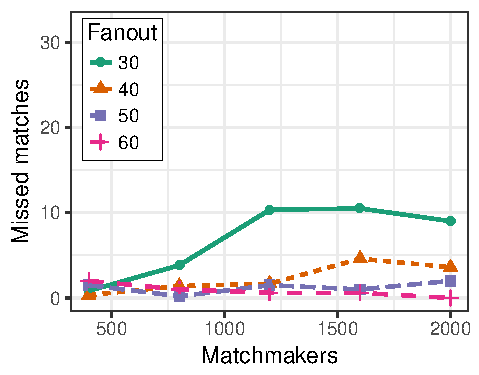
\includegraphics[width=\linewidth]{match/assets/plots/asset_trading_quality.pdf}
		\caption{Matching quality w. different fanouts $ f $}
		\label{fig:asset_trading_quality}
	\end{subfigure}%
	\begin{subfigure}{.5\columnwidth}
		\centering
		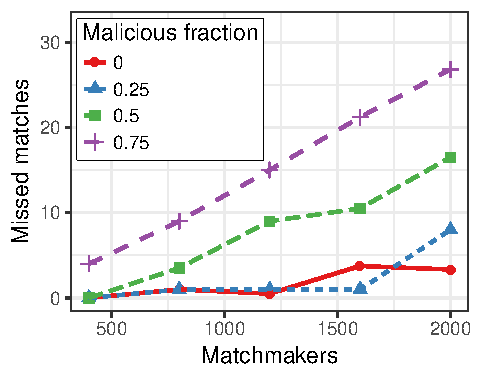
\includegraphics[width=\columnwidth]{match/assets/plots/asset_trading_fairness_fixed.pdf}
		\caption{Impact of selfish matching ($ f = 50 $)}
		\label{fig:asset_trading_fairness_fixed}
	\end{subfigure}\vspace{0.3cm}
	\begin{subfigure}{.5\columnwidth}
		\centering
		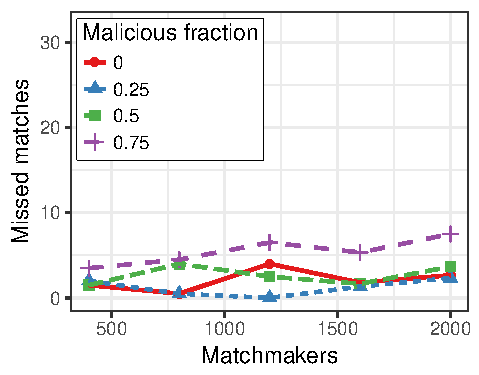
\includegraphics[width=\columnwidth]{match/assets/plots/asset_trading_fairness_adaptive.pdf}
		\caption{Impact of selfish matching (adaptive $ f $)}
		\label{fig:asset_trading_fairness_adaptive}
	\end{subfigure}
	\caption{The matching quality and impact of selfish matching when executing the ride-hailing workload in MATCH, while varying the number of matchmakers. In Figure (b) and (c), the order fanout $ f $ is either fixed  ($ f = 50 $) or adaptive such that $ P(R_{req} \cap R_{off} \neq \emptyset) \geq 0.95 $.}
	\label{fig:asset_trading_experiments}
\end{figure*}

\subsection{Asset Trading Experiments}
\label{sec:asset_trading_experiments}
We now evaluate MATCH in an asset trading domain.
Driven by the popularity of blockchain-based assets, major peer-to-peer markets have emerged to facilitate cryptocurrency exchange between traders~\cite{bentov2019tesseract}.
MATCH enables traders to perform matchmaking of orders themselves in a fair manner, without entrusting their orders to a market operator.
Unlike our previous experiments, the workload used in our upcoming experiments involves offers and requests that be partially fulfilled and are commonly cancelled.
%When deploying MATCH in a domain where digital assets are traded, orders can often be partially fulfilled and are commonly cancelled (e.g., in high-frequency trading).
We conduct the same matching quality and fairness experiments described in Section~\ref{sec:taxi_experiments} with an asset trading workload. % the performance of MATCH is evaluated with an asset trading workload.
%Again, the focus is on the match quality and the impact of malicious matchmakers.

To the best of our knowledge, there is no standardized definition for the matching quality of orders with partial fulfilment.
Therefore, after each experiment with the asset trading workload, we determine the matching quality as follows: all orders that are not cancelled or fulfilled are added to a single order book, starting with the first order created.
When adding these orders to the order book, we sum the number of matches returned by the matching engine, which yields our matching quality.
%For the asset trading experiments, matching quality is defined as the additional number of matches found when adding all open orders to a single order book after the experiment ends, starting with the first order created. %after the experiment by adding all open orders to a single order book, starting with the first order created.
Intuitively, this definition indicates how many additional matches a central matchmaker would have found if it had knowledge of all open orders.
By definition, the matching quality of centralized matchmaking is zero and therefore optimal with FIFO order matching.
In the worst case, our middleware would have missed 6'450 matches, which is the situation where no matchmaker performs any matching.
When running the asset trading workload, the matching engine matches orders according to the \emph{price-time} matching policy~\cite{mavroudis2019libra}.

\textbf{Workload specification.}
The asset trading workload contains buy and sell orders that have been published on the blockchain ledger of BitShares~\cite{schuh2017bitshares}.
BitShares is a blockchain-based decentralized exchange where users can create, issue and trade digital assets.
New orders are submitted to dedicated validator nodes, which include incoming orders in a block on the blockchain.
We have analysed the entire BitShares blockchain since its inception and extracted all buy and sell orders, and order cancellations.
To generate load on our system, we determined when most orders were created for five minutes.
%Next, we take a subset of the orders that result in the highest load (trading activity) for a period of five minutes.
The result is a workload with 942 order cancellations, 12'253 offers and 3'342 requests involving 121 unique asset types.
On average, traders create 52 new orders every second.
Since our dataset does not contain temporal information on order creation and cancellation, we assume that each order is uniformly created in the time interval between the last block and the block that contains this specific order.
We believe this approximates the actual creation timestamp of the order and that this does not skew the experiment results.
Again, there is a 60 seconds experiment cooldown period after the creation of the last order.

\textbf{Matching quality.}
Figure~\ref{fig:asset_trading_quality} shows the matching quality while varying the number of matchmakers and order fanout.
By definition, a centralized approach to matchmaking would not miss any match.
Similar to the matching quality experiment with the ride-hailing workload (see Figure \ref{fig:taxi_quality}), matching quality decreases when there are more matchmakers and the order fanout is static.
It particularly interesting to observe how even a relative low order fanout of 30 results in less than ten missed matches on average (only 0.61\% of the maximum number of missed matches).
Further analysis of the workload reveals that various users create multiple orders for the same asset pair within short time.
Therefore, \texttt{match} messages for such orders received are inserted in multiple match queues, and thus re-used.
Users creating multiple smaller orders with similar specifications are reaching more matchmakers and can potentially negotiate better matches.
%For $ m = 2'000 $ and $ f = 60 $, each completed order required \todo{X} negotiations on average.

%Figure \ref{fig:bitshares_effectiveness_static} and \ref{fig:bitshares_effectiveness_dynamic} show the matching accuracy, both with a static and dynamic order fanout.
%The horizontal axis denotes the number of active matchmakers, and the vertical axis the amount of missed matches.

%Note how the \texttt{FIXEDBC} and \texttt{FIXEDBC+SYNC} policies lead to significantly more missed matches if $ m > 1200 $, compared to \texttt{RANDBC} and \texttt{RANDBC+SYNC} policies.
%The reason for this effect is that there are a few traders who create a large number of orders (there are ten traders whom each create over 100 orders).
%In particular, if the same trader sends their new orders to the same matchmaker every time, it could lead to many missing matches.
%This effect is less pronounced for the \texttt{RANDBC} and \texttt{RANDBC+SYNC} policies.
%Figure \ref{fig:bitshares_effectiveness_dynamic} suggests that differences in matching accuracy with a dynamic order fanout are minimal: on average, all evaluated policies only miss three matches.

\textbf{Impact of selfish matching.}
We demonstrate the effect of malicious matchmakers on the matching quality in our asset trading workload, both with a fixed and adaptive order fanout.
Under the asset trading workload, we model a malicious matchmaker as a node that purposefully does not inform the party behind an incoming order about the match with the best price.
Essentially, a malicious matchmaker \enquote{hides} order book entries from the order creator.
%Instead, the matchmaker intends to re-use this pricing information for one of its own orders later.

Figure~\ref{fig:asset_trading_fairness_fixed} shows the number of missed matches with $ f = 50 $ when increasing $ m $ and varying the $ r $.
More matchmakers negatively impacts the matching quality, although its effect is relatively minor.
In particular, even with $ r = 0.5 $ and $ m = 2'000 $, MATCH only misses less than ten matches on average.
We repeat the experiment while adapting the order fanout such that $ P(R_{req} \cap R_{off} \neq \emptyset) \geq 0.95 $, see Figure~\ref{fig:asset_trading_fairness_adaptive}.
It shows that for all settings, MATCH only misses under ten matches on average.

%\textbf{Message breakdown} -
%TODO

%\textbf{Synchronization batch size} - 
%We now consider the effect of sending more orders during an order book synchronization on the matching accuracy and bandwidth usage, see Figure \ref{fig:bitshares_sync_diff}.
%To observe this effect, we deliberately lowered the value of $ d $ and fixed it to 20 ($ TTL = 2 $, $ fanout = 4 $).
%Note how the \emph{RANDBC} only misses a few matches, even with a low value of $ d $.
%On the other hand, the \emph{NEIGHBC} policy misses a significant amount of matches.
%This is expected since orders are synchronized with neighbouring peers, which is less effective when new orders are always broadcast to the same neighbours.
%Also note that the average bandwidth usage shows a linear increase with the synchronization batch size.

%\begin{table*}[t!]
%	\centering
%	\begin{tabular}{|c | c c c c c c|} 
%		\hline
%		\textbf{Policy} & \textbf{Accuracy} & \textbf{Bandwidth Usage} & \textbf{Fault Tolerance} & \textbf{Fairness} & \textbf{Latency} & \textbf{Load Balancing} \\ \hline
%		Centralized & ++ & ++ & -{}- & -{}- & ++ & -{}- \\
%		FIXEDBC & o & o & + & ++ & - & + \\
%		FIXEDBC+SYNC & + & - & ++ & +  & -{}- & ++ \\ 
%		RANDBC & + & o & + & ++ & - & + \\ 
%		RANDBC+SYNC & ++ & -  & ++ & +  & -{}- & ++ \\ 
%		\hline
%	\end{tabular}
%	\caption{A summary of our middleware evaluation. Each entry in the table indicates performance with respect to an evaluated system property for a specific policy, which can be either very high (++), high (+), adequate (o), low (-) or very low (--).}
%	\label{table:evaluation_summary}
%\end{table*}

%\subsection{Summary}
%We have evaluated six system properties of MATCH with both a ride-hailing and asset trading workload.
%Table~\ref{table:evaluation_summary} summarizes our findings and shows the performance of implemented policies for our evaluated system properties.
%Centralized matchmaking provides good matching accuracy, low bandwidth usage, and low order completion times, compared to decentralized matchmaking.
%However, order completion time in a centralized setting also depends on the geographic location of the matchmaking infrastructure.
%For example, a trader might be geographically distant from the matchmaker and experience higher order completion times as a result.

%In general, the four evaluated decentralized matchmaking policies provide comparable matching accuracy and high fault tolerance, load balancing properties and resistance against unfair matchmakers at the cost of increased bandwidth usage and higher order completion times.
%The specific policy one should adopt highly depends on the trading context and the desired system properties.
%For instance, an additional order completion time of a few seconds is likely tolerated by passengers, whereas the same increase would be impractical in high-frequency trading.
%Similarly, the additional bandwidth usage of decentralized matchmaking has higher consequences when MATCH runs on a mobile phone, in comparison to the situation where MATCH runs on a stationary workstation.
%We believe, however, that the benefits of the decentralized matchmaking model outweigh its deficiencies in many real-world situations, in particular, when low order completion time is not an essential requirement.
%Decentralized matchmaking provides strong fault tolerance, fairness and load balancing, at the cost of order fulfill latency and bandwidth usage.
%The matching accuracy of decentralized matchmaking is competitive compared to the centralized setting.

\begin{figure}[t!]
	\centering
	\begin{subfigure}{.5\columnwidth}
		\centering
		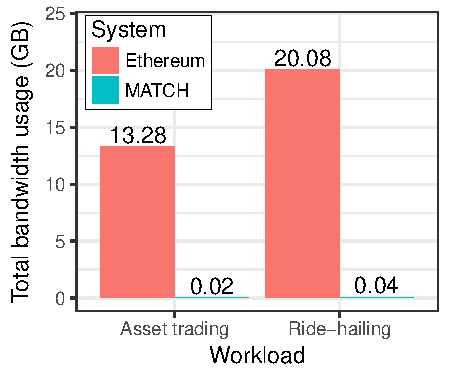
\includegraphics[width=\linewidth]{match/assets/plots/ethereum_bandwidth.pdf}
		\caption{Total bandwidth usage}
		\label{fig:ethereum_bandwidth}
	\end{subfigure}%
	\begin{subfigure}{.5\columnwidth}
		\centering
		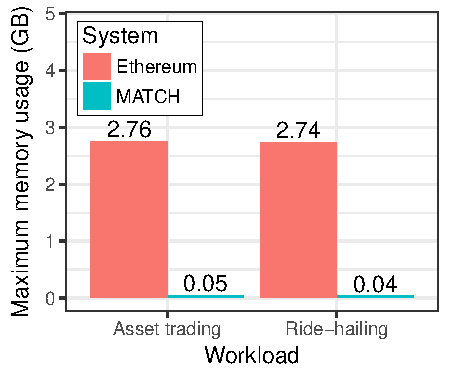
\includegraphics[width=\linewidth]{match/assets/plots/ethereum_memory.pdf}
		\caption{Maximum memory usage}
		\label{fig:ethereum_memory}
	\end{subfigure}\vspace{0.3cm}
	\begin{subfigure}{.5\columnwidth}
		\centering
		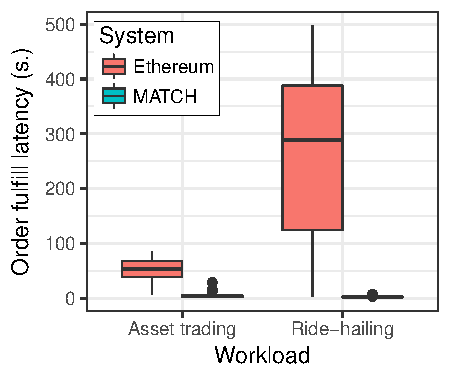
\includegraphics[width=\columnwidth]{match/assets/plots/ethereum_experiment_latencies.pdf}
		\caption{Order fulfil latency}
		\label{fig:ethereum_latencies}
	\end{subfigure}
	\caption{The total bandwidth usage and the distribution of order fulfil latencies of on-chain matchmaking on Ethereum and in MATCH, under the ride-hailing and asset trading workloads.}
	\label{fig:ethereum_experiments}
\end{figure}

\subsection{Comparison with On-chain Matchmaking}
\label{sec:experiments_ethereum}
We compare the bandwidth usage and order fulfil latencies of MATCH with that of matchmaking on an Ethereum blockchain, using both the ride-hailing and asset trading workloads.
%Specifially, we conduct matchmaking on a private Ethereum blockchain.
Ethereum is the most mature blockchain platform that enables the execution of generic-purpose smart contracts, and is the most used platform to deploy smart contracts in general~\cite{wood2014ethereum}.

We setup a private Ethereum network consisting of 400 instances running \texttt{geth}, an Ethereum client written in Go.\footnote{See \url{https://github.com/ethereum/go-ethereum}}
Ethereum uses a Proof-of-Work consensus mechanism in which participants, also called miners, compete to include transactions on the blockchain.
Specifically, each miner continuously solves an algorithmic puzzle and the first miner to find a valid solution to the puzzle, can extend the blockchain with one block with transactions.
We fix \texttt{geth} such that each instance mines on at most one CPU core.
We fix the gas limit (indicating the maximum amount of computation that can be done within a block) to 10'000'000, in line with the public Ethereum network.
To accurately compare the performance of MATCH and Ethereum, we run both workloads in MATCH with 400 instances, and adjust our workload accordingly.
We fix $ m = 400 $, $ f = 30 $ and $ r = 0 $.
Since a smart contract enforces the correct execution of a particular matching policy, we run MATCH with 400 honest matchmakers.

\textbf{Smart contracts.}
For both workloads, we implement a smart contract in the Solidity programming language.
The smart contract for the ride-hailing workload maintains two lists containing open offers and requests.
Submission of a new ride offer and request is done by issuing a transaction with geographic information that invokes the \texttt{ride\_offer} and \texttt{ride\_request} methods in the smart contract, respectively.
Invocation of these methods triggers a loop through the list of active offers or request, and finds the matching order that minimizes the distance between the passenger and driver.
The algorithmic complexity when matching a single offer and request is $ O(n) $ where $ n $ is the number of open requests and offers, respectively.
To avoid computationally expensive trigonometry operations when computing the haversine distance, latitude and longitude coordinates are projected to Universal Transverse Mercator (UTM) coordinates and the Manhattan distance is used as a norm in the smart contract.
This results in an accuracy loss of only 0.35\%.

For the asset trading workload, we adopt an existing and deployed order book implementation.\footnote{See \url{https://github.com/makerdao/maker-otc/tree/master/src}}
This smart contract implements a market to trade digital tokens that reside on the Ethereum blockchain.
Orders are bundled in a limit order book and organized in distinct price levels.
This allows for a strategic search for order matches and avoids the need for a full linear scan through all offers and requests.
This order book organization is predominantly used by financial exchanges.
To quantify the overhead of order matchmaking, we remove the operation that transfers token ownership after matching from the smart contract but leave the implemented price-time matchmaking logic intact.

\textbf{Bandwidth usage.}
We measure the aggregated bandwidth usage of all instance of MATCH and Ethereum, see Figure~\ref{fig:ethereum_bandwidth}.
Ethereum requires over 20GB of network traffic for the ride-hailing workload.
In comparison, MATCH uses dramatically less bandwidth compared to Ethereum-based matchmaking.
MATCH only requires 41.6MB of aggregate network traffic under the ride-haling workload, and 20.7MB under the asset trading workload.
The high bandwidth usage of Ethereum is a direct consequence of the full replication of state.
Specifically, each transaction and block is disseminated to all active Ethereum instances, resulting in a significant amount of network traffic.

\textbf{Memory usage.}
We measure the maximum memory usage of all running MATCH and Ethereum instances, see Figure~\ref{fig:ethereum_memory}.
At peak, Ethereum requires 2.8GB of memory to store pending transactions.
This is partially due to the specifications of the mining algorithm in Ethereum, which requires the storage of a 1GB graph in memory.
Furthermore, each Ethereum instance maintains all unconfirmed transactions and recent blocks in memory.
In comparison, MATCH only requires around 50MB of memory for both workloads, most of which is overhead of the Python interpreter.

\textbf{Order fulfil latencies.}
In Figure~\ref{fig:ethereum_latencies}, we show the time it takes to complete orders in MATCH and Ethereum, for both workloads.
Specifically, this is the time between order creation and order fulfilment.
For the ride-hailing workload, we only consider the completion time of requests made by passengers, since drivers are waiting for incoming requests.
Figure~\ref{fig:ethereum_latencies} shows that the average order completion time of MATCH under the ride-hailing workload is 2.46 seconds and increases under the asset trading workload to 5.02 seconds.
Since users aggregate \texttt{match} messages during the match window, the order fulfil latency in MATCH is at least $ W_{match} $ (which is fixed to two seconds in our experiments).
In comparison, the average order fulfil latency in Ethereum is 258.2 and 53.6 seconds under the ride-hailing and asset trading workload, respectively.
We argue that in a ride-hailing market, the latencies experienced when performing matchmaking on an Ethereum blockchain would be unacceptable for both passengers and drivers.

\begin{figure}[t]
	\centering
	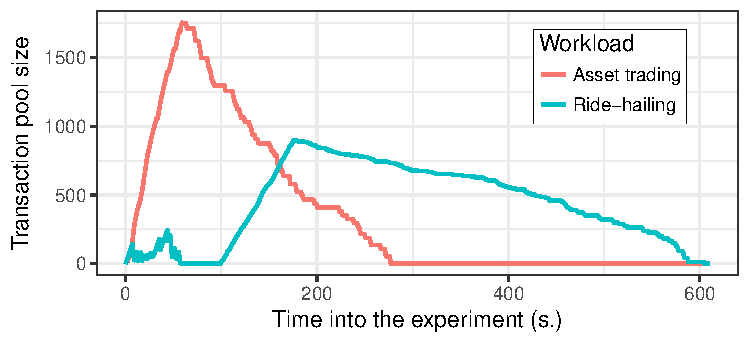
\includegraphics[width=.8\linewidth]{match/assets/plots/tx_pool}
	\caption{The size of the transaction pool during our Ethereum experiments, under the ride-hailing and asset trading workloads.}
	\label{fig:ethereum_tx_pool}
\end{figure}

\textbf{Ethereum transaction pool.}
To further analyse the large differences in order fulfil latencies between MATCH and Ethereum, we visualize the size of the Ethereum transaction pool (as maintained by a single Ethereum instance) during the experiment in Figure~\ref{fig:ethereum_tx_pool}.
This figure shows the time into the experiment on the horizontal axis and the number of transactions in the pool on the vertical axis.
The transaction pool contains transactions that are not yet included in a block on the blockchain by a miner.
Note how Ethereum becomes congested under the asset trading workload quickly after starting the experiment.
Around 70 seconds into the asset trading experiment, the transaction pool contains 1'713 unconfirmed transactions that are buying or selling assets.
285 seconds after the start of this experiments, all orders are included in a block on the Ethereum blockchain.

The ride hailing experiment starts by drivers submitting ride offers to Ethereum instances.
All ride offers are included on the Ethereum blockchain after 58 seconds into the experiment.
Passengers start to submit ride requests 100 seconds into the experiment.
Similar to the asset trading workload, the size increase of the Ethereum transaction pool shows that the blockchain is unable to handle the load of incoming transaction, causing congestion.
180 seconds into the experiment, the number of unconfirmed transactions decreases.
Further inspection of the blockchain reveals that only around ten transactions with a ride request are included in each block.
We explain this behaviour as follows.
In Ethereum, the sum of gas usage of all transactions in a block cannot exceed 10'000'000 gas.
The gas cost of matching ride requests scales with the number of open ride offers and decreases during the experiment since there are less offers to compare with.
Note how after 500 seconds into the ride-hailing experiment, the number of unconfirmed transactions decreases quickly.

%Overall, our comparison experiments highlight the resource costs associated with transparent matchmaking.

\section{Related Work}
Matchmaking (or brokering) is a core concept in publish/subscribe (Pub/Sub) architectures.
In centralized Pub/Sub architectures, a single server brokers incoming messages between publishers and subscribers~\cite{Carzaniga2001DesignAE}.
Decentralized approaches either flood events through the entire network, or route these events based on their topic or content~\cite{banavar1999efficient,carzaniga2004routing}.
In contrast to Pub/Sub systems, MATCH does not ensure that events (orders) are eventually delivered to all subscribers (matchmakers).

%We believe that decentralized, content-based routing of orders (events) can be a promising starting point for an alternative order matching mechanism~\cite{Li2005CompositeSI}.
%Traders then act as publishers and route orders (events) to matchmakers, which subscribe to specific types of orders. % a distributed order book mechanism can be modelled as a content-based publish-subscribe system where subscribers (potential buyers) subscribe to order events generated by publishers (potential sellers).
%However, publish/subscribe architectures aim for eventual delivery to \emph{all} interested subscribers, which is not a scalable approach when many orders are submitted.

Resource allocation, the assignment of compute resources to incoming jobs, also requires matchmaking~\cite{czajkowski1998resource}.
%Various matchmaking architectures have been proposed in the context of resource allocation.
Most work on resource allocation aims to find an optimal assignment between resources and jobs, whereas our work focuses on establishing any match~\cite{ludwig2012matchmaking}.
In this context, we identify two matchmaking approaches described in literature.
The first approach is to use market mechanisms that coordinate the matchmaking process, e.g., by a continuous double auction mechanism~\cite{gomoluch2003market,mihailescu2010distributed,Buyya2002EconomicMF}.
Market-based matching approaches increase allocation efficiency but compromise on computational efficiency since it requires synchronization mechanisms.
The second approach to matchmaking is to deploy one or more dedicated (centralized) brokers~\cite{raman1998matchmaking,frey2002condor,ebrahimi2004matchmaking}.

Motivated by the scalability and load balancing issues of centralized matchmaking, various researchers explored the usage of multiple, independent matchmakers~\cite{azab2008adaptive,edinger2016decentralized,abdullah2010effect,sigdel2005framework}.
Matchmakers usually operate within their own administrative domain, acting as a broker for a specific set of nodes.
%The work of Sigdel et al. specifically addresses load balancing issues and present a hybrid solution where matchmakers are automatically deployed when the system load increases~.
%While comparable to the federated matchmaking model, their architecture lacks scientific evaluation under a realistic workload.
The work of Shafran et al. evaluates a distributed matchmaking model where orders are cached by intermediate agents~\cite{shafran2008towards}.
Their work, however, only considers one-to-one matching.

With the proliferation of blockchain-based tokens, there have been various proposals for matchmaking architectures that complement decentralized exchanges.
These architectures aim to avoid transaction fees and expensive on-chain matchmaking by relying on an off-chain order matching service, and on-chain order execution.
IDEX, an Ethereum-based decentralized exchange, uses a centralized server for order matchmaking~\cite{idex}.
In AirSwap, \emph{indexers} mediate trade between makers, nodes who create an order, and takers, who fulfil existing orders~\cite{swap}. %, and act as matchmakers.
In contrast to MATCH, a user can only send a new order to a single AirSwap indexer.
The 0x protocol uses a similar matchmaking approach since traders send a new order to exactly one matchmaker~\cite{warren20170x}.
The Loopring protocol is similar to the decentralized matching model of MATCH since traders submit orders to one or more \emph{relay nodes}~\cite{loopring}.
The protocol description, however, lacks details on the dissemination strategy of orders to matchmakers.

Auctions are related to order matchmaking since they also provide a mechanism to allocate resources from sellers to buyers.
PeerMart is a decentralized auction mechanism that uses sets of distributed brokers~\cite{haussheer2005decentralized}.
There have been various proposals to run Ethereum-based auctions while preserving the privacy of bidders~\cite{galal2018verifiable,galal2018succinctly}.
Yet, auctions and order matchmaking are different economic primitives with differing goals.
In contrast to order matchmaking, timeframes (and time limitations) are critical in auctions.
Furthermore, auctions have higher security requirements and need (time-bounded) coordination amongst participants, e.g., to determine the winning bidder.

% Focus on economics
%We identify two major differences between our MATCH infrastructure and existing matchmaking infrastructures for blockchain-managed tokens.
%First, MATCH focusses on system properties such as scalability and fault tolerance, whereas related work mostly approaches matchmaking from a governance and economics perspective.
%Second, we noticed that most related work discussed above lacks any scientific grounding and experimental evaluation of the proposed ideas.
%This work is the first to systematically evaluate properties of decentralized order matchmaking, to our best knowledge.

\section{Conclusions}
We have presented MATCH, a decentralized middleware for fair matchmaking in peer-to-peer markets.
Our work addresses fairness concerns associated with the use of in-house, proprietary solutions controlled by a market operator.
In the MATCH protocol, users send new orders to a small, random subset of matchmakers, which inform users about potential matches.
Users then engage in peer-to-peer negotiation about matches with other users.
This approach makes MATCH resilient against matchmakers who deviate from a standard matching policy.
We have devised the MATCH middleware architecture, suitable for deployment in a WAN environment.
%We improved upon existing matchmaking models and introduced the decentralized matchmaking paradigm, where orders are sent to multiple matchmakers and actively shared between them.
%The decentralized matchmaking model yields high fault tolerance and good load balancing, at the cost of additional communication overhead and order fulfill latency.
%We have presented both a novel three-phase matching protocol, based on match notifications and peer-to-peer trade negotiation, and a middleware with effective order dissemination and synchronization policies.
We have experimentally proven resistance against malicious matchmakers in a ride-hailing and asset trading domain, showing that MATCH still establishes high-quality matches.
Our comparison experiments have showed that the resource usage of MATCH is considerably lower compared to that of matchmaking on an Ethereum blockchain.